\documentclass[preprint, 10pt]{elsarticle}

\newcommand{\mcaption}[2]{\caption{\small \em #1}\label{#2}}
\newcommand{\secref}[1]{\ref{#1}}

%\usepackage{algorithmic}
%\usepackage{algorithm}
\usepackage{amsfonts}
\usepackage[fleqn,reqno]{amsmath}
\usepackage{amssymb}
%\usepackage{amsthm}
\usepackage[titletoc]{appendix}
\usepackage{array}
%\usepackage{bm}
%\usepackage{caption}
%\usepackage[usenames]{color}
\usepackage{enumitem}
%\usepackage{epsfig}
%\usepackage{fancybox}
\usepackage{filecontents}
\usepackage[top=1.2in,bottom=1.2in,left=1in, right=1in]{geometry}
\usepackage{graphics}
%%\usepackage{ifthen}
\usepackage{lineno}
%\usepackage{mathrsfs}
%\usepackage{mdframed}
%\usepackage{multirow}
%\usepackage{palatino}
%\usepackage{showkeys} %To see the labels for now.  Will remove later
%\usepackage{stmaryrd}
%\usepackage{subfigure}
%\usepackage{paralist}
\usepackage{pgfplots}
%\usepackage{tabularx}
\usepackage{tikz}
\usepackage{todonotes}
\usetikzlibrary{arrows}
\usepackage{comment}

%%%%%%  pdftex  %%%%%%%%%%%%%%%%%%%%%%%%%%%%%%%%%%%%%%%%%%%%%%%%%%%%%%
\usepackage[pagebackref=false,bookmarks=false]{hyperref} 

\hypersetup{
  bookmarksnumbered=true,
  bookmarksopen=false,
  hypertexnames=false,      
  breaklinks=true,          
  unicode=false,
  pdffitwindow=true,        
  pdfnewwindow=true,        
  colorlinks=true,         
  linkcolor=dblue,
  anchorcolor=red,
  citecolor=dorange,
  filecolor=magenta,
  urlcolor=dblue,
  pdfstartview = FitH,
  pdfkeywords = {},
  pdfcreator = {LaTeX with hyperref package}
}



\newcommand{\bd}{{\partial}}
\newcommand{\bigO}{{\mathcal{O}}}
\newcommand{\cc}{{\mathbf{c}}}
\newcommand{\DD}{{\mathcal{D}}}
\newcommand{\eeta}{{\boldsymbol\eta}}
\newcommand{\ff}{{\mathbf{f}}}
\newcommand{\grad}{{\nabla}}
\newcommand{\II}{{\mathbf{I}}}
\newcommand{\iin}{\mathrm{in}}
\newcommand{\llambda}{{\boldsymbol\lambda}}
\newcommand{\nn}{{\mathbf{n}}}
\newcommand{\NN}{{\mathcal{N}}}
\newcommand{\out}{\mathrm{out}}
\newcommand{\rr}{{\mathbf{r}}}
\newcommand{\RR}{{\mathbb{R}}}
\renewcommand{\ss}{{\mathbf{s}}}
\newcommand{\ssigma}{{\boldsymbol\sigma}}
\newcommand{\tar}{\mathrm{tar}}
\newcommand{\uu}{{\mathbf{u}}}
\newcommand{\UU}{{\mathbf{U}}}
\newcommand{\vv}{{\mathbf{v}}}
\newcommand{\xx}{{\mathbf{x}}}
\newcommand{\xxi}{{\boldsymbol{\xi}}}
\newcommand{\yy}{{\mathbf{y}}}

\def\gap{\hspace*{.2in}}

% Derivatives
\newcommand{\pderiv}[2]{\frac{\partial #1}{\partial #2}}
\newcommand{\tderiv}[2]{\frac{d #1}{d #2}}
\newcommand{\ppd}[2]{\frac{\partial^2 #1}{{\partial #2}^2}}

% Nick's commands
\newcommand{\vsp}[1]{\vspace{#1 pc} \noindent}
\newcommand{\abs}[1]{\lvert #1 \rvert}
\newcommand{\mean}[1]{\left< #1 \right>}
\newcommand{\thL}{$\theta$--$L$}
\newcommand{\eps}{\varepsilon}
\newcommand{\Vn}{V_n}
\newcommand{\Vs}{V_s}
\newcommand{\atau}{\abs{\tau}}
\newcommand{\thalpha}{\pderiv{\theta}{\alpha}}
\newcommand{\elfun}{\zeta}
\newcommand{\thhat}{\hat{\theta}}
\newcommand{\Dt}{\Delta t}
\newcommand{\NLterm}{\mathcal{N}}
\newcommand{\Mterm}{\mathcal{M}}
\newcommand{\FourierSum}{ \sum_{k = -N_\iin /2}^{N_\iin /2-1} }
\newcommand{\atausig}{\atau^{(\sigma)}}
\newcommand{\Vnsig}{\Vn^{(\sigma)}}
\newcommand{\Vssig}{\Vs^{(\sigma)}}


\newcommand{\tauD}[1]{\tau_{#1\text{D}}}
\newcommand{\atauD}[1]{\abs{\tau_{#1\text{D}}}}

\begin{document}

\title{Viscous Erosion in Porous Media}

\author[Bryan]{Bryan D.~Quaife}
\author[Nick]{M.~Nicholas J.~Moore}
\address[Nick]{Department of Mathematics and Geophysical Fluid Dynamics Institute, Florida State University, Tallahassee, FL, 32306.}
\address[Bryan]{Department of Scientific Computing and Geophysical Fluid Dynamics Institute, Florida State University, Tallahassee, FL, 32306.}

\begin{abstract} 
We consider two dimensional eroding bodies in Stokes flow
\end{abstract}

\begin{keyword}
  Stokes flow \sep Erosion \sep Boundary integral method \sep Shear
  stress \sep {\thL} formulation
\end{keyword}

\maketitle

%%%%%%%%%%%%%%%%%%%%%%%%%%%%%%%%%%%%%%%%%%%%%%%%%%%%%%%%%%%%%%%%%%%%%%%
\section{Introduction\label{s:intro}}
Erosion is a fluid-mechanical process that is responsible for a variety
of phenomena in geophysical fluids and other processes.  For example,
wind erosion causes sand dunes to be  longer on the windward
side~\cite{han1969}, and erosion is responsible for branching structures
of streams and rivers~\cite{coh-dev-sey-yi-szy-rot2015}.  Erosion is
also important in the biophysical community. Plaque erosion in arteries
is key to understanding heart disease~\cite{sha2002,
gro-gij-van-fer-hat-van-yua-wen2007}, and the separation of biofilms can
be explained by erosion~\cite{pic-van-hei2000}.  Another application,
which motivates the current work, is erosion caused by groundwater flow.
Here, a slow moving fluid erodes channels in the ground, and this
affects the fluid transport.  In all these examples, there is a feedback
process between the flow and the eroding bodies---the shape of the
bodies affect the flow, while the flow changes the shape by fluidizing
each body.  This fluid-mechanical feedback system has been simulated in
idealized cases such as a single eroding two-dimensional body in a
uniform flow~\cite{moo-ris-chi-zha-she2013} or a single mobile eroding
three-dimensional body~\cite{mit-spa2016}. However, to better understand
the effect of erosion on groundwater flow, multiply-connected domains
must be considered.  Here we simulate two-dimensional erosion, in
multiply-connected domain such as the porous geometry of many
groundwater flows (Fig.~\ref{fig:50bodies}).

Because of the length and velocity scales of groundwater flow, we
restrict our attention to small Reynolds number flows.  For groundwater
flow, Darcy's law is often used, but this does not resolve the pore
structure and assumes a homogeneous geometry which is often not valid.
Instead, we use the incompressible Stokes equations to represent the
flow, and the individual pores are resolved which results in a complex
multiply-connected geometry.  A boundary integral equation is
well-suited for solving the incompressible Stokes equations in a complex
geometry since it can resolve individual grains and the non-negligible
interactions between bodies are resolved. Moreover, high-order accuracy
and computational efficiency are obtained. To link the eroding body and
fluid dynamics, the body is eroded in the normal direction at a rate
that is proportional to the magnitude of the shear
stress~\cite{ris-moo-chi-she-zha2012}.  Tracking the interface of
fluid-structure interaction problems with a long time horizon is
particularly---the mesh is often distorted and tangled by the dynamics
and regions of high curvature develop.  These two issues are resolved
by, first, introducing a tangential velocity field to maintain a grid
that is equispaced in arclength, but that does not affect the dynamics,
and, second, a curvature penalization term.  Furthermore, the frame of
reference is changed to \thL~variables so that the curvature term
appears as a linear diffusive term that can easily be treated implicitly
to avoid stiffness.

In addition to simulating the eroding grains, the flow is further
characterized by computing the vorticity in the flow.  The vorticity is
particularly insightful since it is identical to the shear stress on
no-slip boundaries in the Stokesian limit.  Therefore, by computing the
vorticity, we are able to locate regions where the erosion rates will be
fastest or slowest.

%%%%%%%%%%%%%%%%%%%%%%%%%%%%%%%%%%%%%%%%%%%%%%%%%%%%%%%%%%%%%%%%%%%%%%%
\paragraph{Contributions} The present study develops numerical methods
to simulate erosion of multiply-connected two-dimensional geometries.
Since groundwater flow occurs at small spatial and velocity scales, we
assume the flow is viscous (ie.~zero Reynolds number).  By allowing for
complex multiply-connected domains, we capture the effect that
interacting bodies have on erosion, and the grains in the flow are
individually resolved rather than homogenized.  We start by validating
our method on a single circular body placed symmetrically in a pipe
flow.  By artificially fixing the area of the body as a function of
time, we are able to characterize the long-time behavior of the shape
and the resulting flow and compare these results with analytical
results.  Then, we compute the vorticity of erosion in
multiply-connected geometries to better characterize erosion in porous
media. 

To create high-fidelity and computationally efficient numerical methods,
two fast and accurate methods are employed.  First, the fluid equations
and the erosion rate (shear stress) are efficiently solved with spectral
accuracy by using a fast multipole accelerated boundary integral
equation method.  Given the rate of erosion, the shape is integrated in
time with second-order accuracy.  All spatial derivatives are be
computed in Fourier space, resulting in spectral accuracy in space.
Then, to further visualize the effect of erosion, we compute the
vorticity of the flow (Fig.~\ref{fig:50bodies}) to visualize regions
of high and low erosion.

A challenge with erosion is that it creates corners at points on the
body where the shear stress vanishes.  While recent work does allow for
integral equation methods to resolve corners, we employ a different
method.  First, we add a regularization term to the shear stress to
penalize regions of high curvature.  Second, we apply a Gaussian filter
to smooth the absolute value of the shear stress before the body shape
is updated.

%%%%%%%%%%%%%%%%%%%%%%%%%%%%%%%%%%%%%%%%%%%%%%%%%%%%%%%%%%%%%%%%%%%%%%%
\paragraph{Limitations} There are two main limitations of the current
work.  First, the flow is assumed to be two-dimensional.  However, by
assuming that the flow is two-dimensional, we are able to simulate the
erosion of more bodies and with higher resolution than would be
available in three dimensions.  Moreover, several flows can be described
to good accuracy under a two-dimensional approximation, but certain
phenomena occur only in three dimensions.  Extending the current work to
three dimensions is possible with a boundary integral equation
formulation.  In particular, the fluid solvers exist~\cite{mal-bir2015},
and the main challenges of a BIE solver have been addressed by other
groups including surface representation~\cite{yin-bir-zor2006,
vee-rah-bir-zor2011}, near-singular integration~\cite{yin-bir-zor2006,
kli-tor2016b}, and fast summation methods~\cite{yin-bir-zor2004,
ros-ols2015}.  The more significant challenge of extending our work to
three dimensions is guaranteeing that the mesh does not become
distorted, which can be done, for example, by using an extension of the
two-dimensional {\thL} formulation~\cite{amb-sie-tlu2013}.

The second limitation is that the eroding bodies are fixed.  Mitchell
and Spagnolie~\cite{mit-spa2016} simulate a single mobile eroding body
in three dimensions~\cite{mit-spa2016}, but additional challenges are
caused when there are multiple bodies. In particular, especially in
dense suspensions, bodies can become extremely close to one another, and
the interaction between the bodies is difficult to resolve unless the
underlying mesh is refined to levels that are intractable. In future
work we plan to consider mobile eroding bodies, but include a small
force and torque so that unphysical contact is
avoided~\cite{lu-rah-zor2017}.

%%%%%%%%%%%%%%%%%%%%%%%%%%%%%%%%%%%%%%%%%%%%%%%%%%%%%%%%%%%%%%%%%%%%%%%
\paragraph{Related work} Simulating eroding bodies has been studied
analytically, experimentally, and numerically.  Because of the scales
involves with geophysical flows, most of these works consider high
Reynolds number flows.  For instance, the experimental work of Moore et
al.~\cite{moo-ris-chi-zha-she2013} considers on the order of $10^4$.
For low Reynolds number flows, Mitchell and Spagnolie~\cite{mit-spa2016}
simulate the erosion of a mobile body in three dimensions, but they only
consider single body.  

Mitchell and Spagnolie~\cite{mit-spa2016} formulate the traction jump as
a DLP using Lorentz Reciprocal Theorem so that additional layer
potentials have to be evaluated.  That is, they never find the density
function.

The effect of erosion on a geometry is quite rich.  For instance, it has
been hypothesized and numerically observed that the erosion leads to a
shear stress that is uniform on the body which results in a uniform
erosion rate.  The shape that has a uniform shear stress is analyzed in
three dimensions by Montenegro-Johnson and Lauga~\cite{mon-lau2015}
which is an extension of the analysis done by Pironneau~\cite{pir1973}
to find a Stokesian drag minimizing shape.  However, the effect of
erosion on a porous media is less understood.  With the methods
developed in this paper, quantities such as the total drag across a
porous region as a function of time can be computed in future work.



To simulate multiple bodies, it is essential to resolve the nonlocal
effects between the different bodies.  In this work, these interactions
are included with high-order accuracy by using an integral equation
method.  Integral equations have been used extensively to simulate
viscous fluids in complex geometries.  One particular application are
particulate flows, such as bubbles or droplets, and the classic book of
Pozrikidis~\cite{poz1992} describes boundary integral formulations for
such problems.

Several groups consider the optimal body in a Stokes fluid that
optimizes some quantity.  For example, Pironneau~\cite{pir1973} found
the axisymmetric shape of a fixed volume body that minimizes drag is
similar to an American football with an opening angle of 60 degrees, and
this shape corresponds to a body with constant surface vorticity.  This
analysis is taken further by Montenegro-Johnson and
Lauga~\cite{mon-lau2015} where the optimal axisymmetric shape of fixed
surface area is computed.  We include a similar calculation for the
two-dimensional Stokes equations, and the resulting shape agrees with
our numerical solution. 

\todo[inline]{Dump of text}
Other models for erosion include ones that use an erosion rate that is
proportional to a power of the magnitude of the shear
stress~\cite{par-izu2000}, or ones that use a critical shear stress
below which erosion does not occur~\cite{lag2000}.
\todo[inline]{Dump of text}



%%%%%%%%%%%%%%%%%%%%%%%%%%%%%%%%%%%%%%%%%%%%%%%%%%%%%%%%%%%%%%%%%%%%%%%
\paragraph{Outline of the paper} In Section~\ref{s:formulation}, we
describe the governing equations for both the fluid and describe the
erosion model using a \thL~framework.  In Section~\ref{s:method}, the
numerical methods in both space and time are described.
Section~\ref{s:results} gives several numerical examples.  Finally,
concluding remarks are made in Section~\ref{s:conclusions}

%^^^^^^^^^^^^^^^^^^^^^^^^^^^^^^%
\begin{figure}%[htbp]
\begin{center}
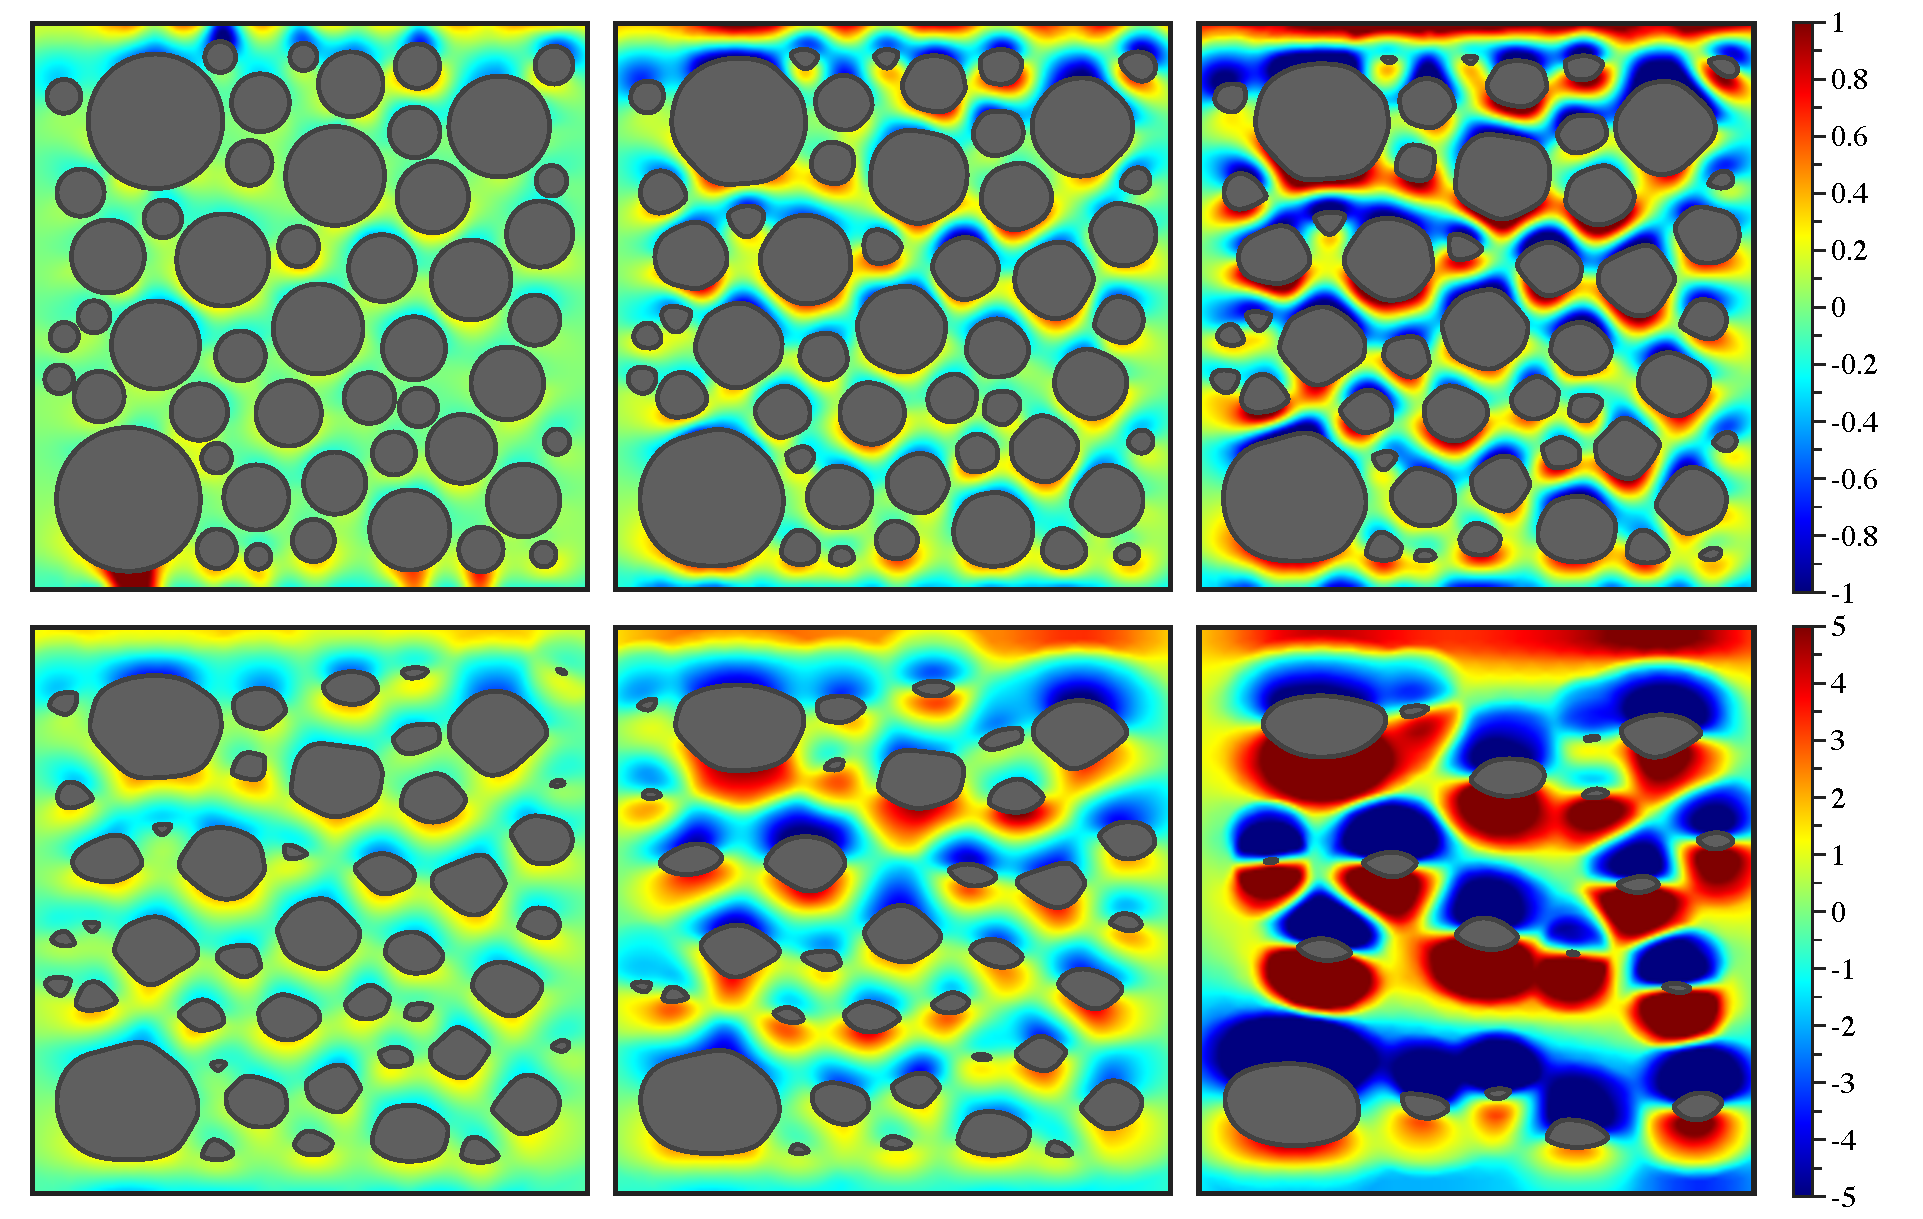
\includegraphics[width = 0.9 \textwidth]{./figs/50bod.pdf}
\caption{\label{fig:50bodies} A time lapse of 50 bodies eroding in a
viscous flow.  The boundary conditions are a constant pressure drop that
creates a flow from the left to right.  The rate of erosion is
proportional to the shear stress which is equivalent to the vorticity
evaluated on the bodies.  The colors represent the vorticity, so regions
with large vorticity (in magnitude) are regions where the flow will
erode the fastest.}
\end{center}
\end{figure}
 %^^^^^^^^^^^^^^^^^^^^^^^^^^^^^^%
% Figure generated from data file 50circ512p5, 
%which uses 50circ512.in with epsfac = 30, sigfac = 10, dt = 1e-4, fixpdrop = 1


%%%%%%%%%%%%%%%%%%%%%%%%%%%%%%%%%%%%%%%%%%%%%%%%%%%%%%%%%%%%%%%%%%%%%%%
\section{Formulation}
\label{s:formulation}
We start by defining the main variables used to model erosion.  We only
consider flows that are confined by a solid wall $\Gamma$ that encloses
$M$ eroding bodies.  The bodies are denoted as $\gamma_\ell$,
$\ell=1,\ldots,M$, and we write $\gamma = \gamma_1 \cup \cdots \cup
\gamma_M$.  Neglecting inertial forces, the dynamics of the fluid is
fully characterized by the position of the bodies $\xx_\ell(s,t) \in
\gamma_\ell$, where $s$ is the arclength and $t$ is time.  Given
$\xx_\ell(s,t)$, $\ell=1,\ldots,M$, derived variables include the fluid
velocity $\uu$, the pressure $p$, and the shear stress $\tau$.   On the
bounding wall, we prescribe a velocity $\UU(\xx,t)$.  Then, the
governing equations are
\begin{equation}
\label{eqn:erosionModel}
\begin{split}
  \mu \Delta \uu = \grad p, &\hspace{20pt} \xx \in \Omega, \gap &&\mbox{conservation
of momentum}\\
\grad \cdot \uu = 0, &\hspace{20pt} \xx \in \Omega, \gap
&&\mbox{\em conservation of mass} \\
\uu = 0, &\hspace{20pt} \xx \in \gamma, \gap &&\mbox{\em no slip on the
bodies} \\
\uu = \UU, &\hspace{20pt} \xx \in \Gamma, \gap &&\mbox{\em outer wall
velocity} \\
\Vn = \abs{\tau}, &\hspace{20pt} \xx \in \gamma,
&&\mbox{\em erosion model},
\end{split}
\end{equation}
where $\Vn$ is the normal velocity of the interface and $\mu$ is the
fluid viscosity.  The outer wall is formed by rounding off the corners
of $[-3,3] \times [-1,1]$, and we enforce the Hagen-Poiseuille flow
\begin{align*}
  \UU(\xx) = \umax (1-y^2,0), \quad \xx \in \Gamma,
\end{align*}
where $U$ sets the maximum of the imposed Poiseuille flow. Often, we
will simply set $U=1$, but in some instances we change $U$ dynamically
to enforce that the pressure drop across the computational cell is
constant as bodies erode within it.  The boundary of the fluid domain is
$\bd\Omega = \gamma_1 \cup \cdots \cup \gamma_M \cup \Gamma$.  To
minimize the boundary effects of the inflow and outflow, we only place
bodies in the center third, $[-1,1] \times [-1,1]$, of the fluid domain.
\begin{figure}[htpb]
  \centering
  \begin{tikzpicture}[scale=1.5] 

\begin{axis}[ 
axis equal image, 
scale only axis, 
xmin=-3.04, 
xmax=3.6, 
ymin=-1.1, 
ymax=1.1, 
hide axis, 
] 

\addplot [color=black,dashed,line width=1] coordinates{ 
  (-1,-1)
  (-1,+1)
}; 

\addplot [color=black,dashed,line width=1] coordinates{ 
  (1,-1)
  (1,+1)
}; 

\addplot [color=black,solid,line width=2] coordinates{ 
(3.0000e+00,0.0000e+00)
(3.0000e+00,2.4549e-02)
(3.0000e+00,4.9127e-02)
(3.0000e+00,7.3764e-02)
(3.0000e+00,9.8491e-02)
(3.0000e+00,1.2334e-01)
(3.0000e+00,1.4834e-01)
(3.0000e+00,1.7352e-01)
(3.0000e+00,1.9891e-01)
(3.0000e+00,2.2456e-01)
(3.0000e+00,2.5049e-01)
(3.0000e+00,2.7674e-01)
(3.0000e+00,3.0334e-01)
(2.9999e+00,3.3035e-01)
(2.9999e+00,3.5779e-01)
(2.9998e+00,3.8572e-01)
(2.9997e+00,4.1417e-01)
(2.9994e+00,4.4319e-01)
(2.9991e+00,4.7282e-01)
(2.9985e+00,5.0310e-01)
(2.9975e+00,5.3407e-01)
(2.9960e+00,5.6575e-01)
(2.9938e+00,5.9814e-01)
(2.9904e+00,6.3123e-01)
(2.9854e+00,6.6493e-01)
(2.9780e+00,6.9912e-01)
(2.9673e+00,7.3358e-01)
(2.9520e+00,7.6793e-01)
(2.9306e+00,8.0171e-01)
(2.9014e+00,8.3425e-01)
(2.8625e+00,8.6481e-01)
(2.8126e+00,8.9262e-01)
(2.7510e+00,9.1700e-01)
(2.6779e+00,9.3755e-01)
(2.5944e+00,9.5418e-01)
(2.5028e+00,9.6713e-01)
(2.4051e+00,9.7688e-01)
(2.3038e+00,9.8402e-01)
(2.2007e+00,9.8911e-01)
(2.0974e+00,9.9268e-01)
(1.9948e+00,9.9514e-01)
(1.8937e+00,9.9681e-01)
(1.7944e+00,9.9794e-01)
(1.6972e+00,9.9868e-01)
(1.6022e+00,9.9917e-01)
(1.5093e+00,9.9949e-01)
(1.4185e+00,9.9969e-01)
(1.3296e+00,9.9981e-01)
(1.2425e+00,9.9989e-01)
(1.1572e+00,9.9994e-01)
(1.0734e+00,9.9997e-01)
(9.9105e-01,9.9998e-01)
(9.1003e-01,9.9999e-01)
(8.3021e-01,1.0000e+00)
(7.5146e-01,1.0000e+00)
(6.7367e-01,1.0000e+00)
(5.9674e-01,1.0000e+00)
(5.2055e-01,1.0000e+00)
(4.4501e-01,1.0000e+00)
(3.7001e-01,1.0000e+00)
(2.9547e-01,1.0000e+00)
(2.2129e-01,1.0000e+00)
(1.4738e-01,1.0000e+00)
(7.3646e-02,1.0000e+00)
(1.8370e-16,1.0000e+00)
(-7.3646e-02,1.0000e+00)
(-1.4738e-01,1.0000e+00)
(-2.2129e-01,1.0000e+00)
(-2.9547e-01,1.0000e+00)
(-3.7001e-01,1.0000e+00)
(-4.4501e-01,1.0000e+00)
(-5.2055e-01,1.0000e+00)
(-5.9674e-01,1.0000e+00)
(-6.7367e-01,1.0000e+00)
(-7.5146e-01,1.0000e+00)
(-8.3021e-01,1.0000e+00)
(-9.1003e-01,9.9999e-01)
(-9.9105e-01,9.9998e-01)
(-1.0734e+00,9.9997e-01)
(-1.1572e+00,9.9994e-01)
(-1.2425e+00,9.9989e-01)
(-1.3296e+00,9.9981e-01)
(-1.4185e+00,9.9969e-01)
(-1.5093e+00,9.9949e-01)
(-1.6022e+00,9.9917e-01)
(-1.6972e+00,9.9868e-01)
(-1.7944e+00,9.9794e-01)
(-1.8937e+00,9.9681e-01)
(-1.9948e+00,9.9514e-01)
(-2.0974e+00,9.9268e-01)
(-2.2007e+00,9.8911e-01)
(-2.3038e+00,9.8402e-01)
(-2.4051e+00,9.7688e-01)
(-2.5028e+00,9.6713e-01)
(-2.5944e+00,9.5418e-01)
(-2.6779e+00,9.3755e-01)
(-2.7510e+00,9.1700e-01)
(-2.8126e+00,8.9262e-01)
(-2.8625e+00,8.6481e-01)
(-2.9014e+00,8.3425e-01)
(-2.9306e+00,8.0171e-01)
(-2.9520e+00,7.6793e-01)
(-2.9673e+00,7.3358e-01)
(-2.9780e+00,6.9912e-01)
(-2.9854e+00,6.6493e-01)
(-2.9904e+00,6.3123e-01)
(-2.9938e+00,5.9814e-01)
(-2.9960e+00,5.6575e-01)
(-2.9975e+00,5.3407e-01)
(-2.9985e+00,5.0310e-01)
(-2.9991e+00,4.7282e-01)
(-2.9994e+00,4.4319e-01)
(-2.9997e+00,4.1417e-01)
(-2.9998e+00,3.8572e-01)
(-2.9999e+00,3.5779e-01)
(-2.9999e+00,3.3035e-01)
(-3.0000e+00,3.0334e-01)
(-3.0000e+00,2.7674e-01)
(-3.0000e+00,2.5049e-01)
(-3.0000e+00,2.2456e-01)
(-3.0000e+00,1.9891e-01)
(-3.0000e+00,1.7352e-01)
(-3.0000e+00,1.4834e-01)
(-3.0000e+00,1.2334e-01)
(-3.0000e+00,9.8491e-02)
(-3.0000e+00,7.3764e-02)
(-3.0000e+00,4.9127e-02)
(-3.0000e+00,2.4549e-02)
(-3.0000e+00,1.2246e-16)
(-3.0000e+00,-2.4549e-02)
(-3.0000e+00,-4.9127e-02)
(-3.0000e+00,-7.3764e-02)
(-3.0000e+00,-9.8491e-02)
(-3.0000e+00,-1.2334e-01)
(-3.0000e+00,-1.4834e-01)
(-3.0000e+00,-1.7352e-01)
(-3.0000e+00,-1.9891e-01)
(-3.0000e+00,-2.2456e-01)
(-3.0000e+00,-2.5049e-01)
(-3.0000e+00,-2.7674e-01)
(-3.0000e+00,-3.0334e-01)
(-2.9999e+00,-3.3035e-01)
(-2.9999e+00,-3.5779e-01)
(-2.9998e+00,-3.8572e-01)
(-2.9997e+00,-4.1417e-01)
(-2.9994e+00,-4.4319e-01)
(-2.9991e+00,-4.7282e-01)
(-2.9985e+00,-5.0310e-01)
(-2.9975e+00,-5.3407e-01)
(-2.9960e+00,-5.6575e-01)
(-2.9938e+00,-5.9814e-01)
(-2.9904e+00,-6.3123e-01)
(-2.9854e+00,-6.6493e-01)
(-2.9780e+00,-6.9912e-01)
(-2.9673e+00,-7.3358e-01)
(-2.9520e+00,-7.6793e-01)
(-2.9306e+00,-8.0171e-01)
(-2.9014e+00,-8.3425e-01)
(-2.8625e+00,-8.6481e-01)
(-2.8126e+00,-8.9262e-01)
(-2.7510e+00,-9.1700e-01)
(-2.6779e+00,-9.3755e-01)
(-2.5944e+00,-9.5418e-01)
(-2.5028e+00,-9.6713e-01)
(-2.4051e+00,-9.7688e-01)
(-2.3038e+00,-9.8402e-01)
(-2.2007e+00,-9.8911e-01)
(-2.0974e+00,-9.9268e-01)
(-1.9948e+00,-9.9514e-01)
(-1.8937e+00,-9.9681e-01)
(-1.7944e+00,-9.9794e-01)
(-1.6972e+00,-9.9868e-01)
(-1.6022e+00,-9.9917e-01)
(-1.5093e+00,-9.9949e-01)
(-1.4185e+00,-9.9969e-01)
(-1.3296e+00,-9.9981e-01)
(-1.2425e+00,-9.9989e-01)
(-1.1572e+00,-9.9994e-01)
(-1.0734e+00,-9.9997e-01)
(-9.9105e-01,-9.9998e-01)
(-9.1003e-01,-9.9999e-01)
(-8.3021e-01,-1.0000e+00)
(-7.5146e-01,-1.0000e+00)
(-6.7367e-01,-1.0000e+00)
(-5.9674e-01,-1.0000e+00)
(-5.2055e-01,-1.0000e+00)
(-4.4501e-01,-1.0000e+00)
(-3.7001e-01,-1.0000e+00)
(-2.9547e-01,-1.0000e+00)
(-2.2129e-01,-1.0000e+00)
(-1.4738e-01,-1.0000e+00)
(-7.3646e-02,-1.0000e+00)
(-5.5109e-16,-1.0000e+00)
(7.3646e-02,-1.0000e+00)
(1.4738e-01,-1.0000e+00)
(2.2129e-01,-1.0000e+00)
(2.9547e-01,-1.0000e+00)
(3.7001e-01,-1.0000e+00)
(4.4501e-01,-1.0000e+00)
(5.2055e-01,-1.0000e+00)
(5.9674e-01,-1.0000e+00)
(6.7367e-01,-1.0000e+00)
(7.5146e-01,-1.0000e+00)
(8.3021e-01,-1.0000e+00)
(9.1003e-01,-9.9999e-01)
(9.9105e-01,-9.9998e-01)
(1.0734e+00,-9.9997e-01)
(1.1572e+00,-9.9994e-01)
(1.2425e+00,-9.9989e-01)
(1.3296e+00,-9.9981e-01)
(1.4185e+00,-9.9969e-01)
(1.5093e+00,-9.9949e-01)
(1.6022e+00,-9.9917e-01)
(1.6972e+00,-9.9868e-01)
(1.7944e+00,-9.9794e-01)
(1.8937e+00,-9.9681e-01)
(1.9948e+00,-9.9514e-01)
(2.0974e+00,-9.9268e-01)
(2.2007e+00,-9.8911e-01)
(2.3038e+00,-9.8402e-01)
(2.4051e+00,-9.7688e-01)
(2.5028e+00,-9.6713e-01)
(2.5944e+00,-9.5418e-01)
(2.6779e+00,-9.3755e-01)
(2.7510e+00,-9.1700e-01)
(2.8126e+00,-8.9262e-01)
(2.8625e+00,-8.6481e-01)
(2.9014e+00,-8.3425e-01)
(2.9306e+00,-8.0171e-01)
(2.9520e+00,-7.6793e-01)
(2.9673e+00,-7.3358e-01)
(2.9780e+00,-6.9912e-01)
(2.9854e+00,-6.6493e-01)
(2.9904e+00,-6.3123e-01)
(2.9938e+00,-5.9814e-01)
(2.9960e+00,-5.6575e-01)
(2.9975e+00,-5.3407e-01)
(2.9985e+00,-5.0310e-01)
(2.9991e+00,-4.7282e-01)
(2.9994e+00,-4.4319e-01)
(2.9997e+00,-4.1417e-01)
(2.9998e+00,-3.8572e-01)
(2.9999e+00,-3.5779e-01)
(2.9999e+00,-3.3035e-01)
(3.0000e+00,-3.0334e-01)
(3.0000e+00,-2.7674e-01)
(3.0000e+00,-2.5049e-01)
(3.0000e+00,-2.2456e-01)
(3.0000e+00,-1.9891e-01)
(3.0000e+00,-1.7352e-01)
(3.0000e+00,-1.4834e-01)
(3.0000e+00,-1.2334e-01)
(3.0000e+00,-9.8491e-02)
(3.0000e+00,-7.3764e-02)
(3.0000e+00,-4.9127e-02)
(3.0000e+00,-2.4549e-02)
(3.0000e+00,0.0000e+00)
}; 

\addplot [color=black,solid,fill] coordinates{ 
(5.0000e-01,0.0000e+00)
(4.9759e-01,4.9009e-02)
(4.9039e-01,9.7545e-02)
(4.7847e-01,1.4514e-01)
(4.6194e-01,1.9134e-01)
(4.4096e-01,2.3570e-01)
(4.1573e-01,2.7779e-01)
(3.8651e-01,3.1720e-01)
(3.5355e-01,3.5355e-01)
(3.1720e-01,3.8651e-01)
(2.7779e-01,4.1573e-01)
(2.3570e-01,4.4096e-01)
(1.9134e-01,4.6194e-01)
(1.4514e-01,4.7847e-01)
(9.7545e-02,4.9039e-01)
(4.9009e-02,4.9759e-01)
(3.0616e-17,5.0000e-01)
(-4.9009e-02,4.9759e-01)
(-9.7545e-02,4.9039e-01)
(-1.4514e-01,4.7847e-01)
(-1.9134e-01,4.6194e-01)
(-2.3570e-01,4.4096e-01)
(-2.7779e-01,4.1573e-01)
(-3.1720e-01,3.8651e-01)
(-3.5355e-01,3.5355e-01)
(-3.8651e-01,3.1720e-01)
(-4.1573e-01,2.7779e-01)
(-4.4096e-01,2.3570e-01)
(-4.6194e-01,1.9134e-01)
(-4.7847e-01,1.4514e-01)
(-4.9039e-01,9.7545e-02)
(-4.9759e-01,4.9009e-02)
(-5.0000e-01,6.1232e-17)
(-4.9759e-01,-4.9009e-02)
(-4.9039e-01,-9.7545e-02)
(-4.7847e-01,-1.4514e-01)
(-4.6194e-01,-1.9134e-01)
(-4.4096e-01,-2.3570e-01)
(-4.1573e-01,-2.7779e-01)
(-3.8651e-01,-3.1720e-01)
(-3.5355e-01,-3.5355e-01)
(-3.1720e-01,-3.8651e-01)
(-2.7779e-01,-4.1573e-01)
(-2.3570e-01,-4.4096e-01)
(-1.9134e-01,-4.6194e-01)
(-1.4514e-01,-4.7847e-01)
(-9.7545e-02,-4.9039e-01)
(-4.9009e-02,-4.9759e-01)
(-9.1849e-17,-5.0000e-01)
(4.9009e-02,-4.9759e-01)
(9.7545e-02,-4.9039e-01)
(1.4514e-01,-4.7847e-01)
(1.9134e-01,-4.6194e-01)
(2.3570e-01,-4.4096e-01)
(2.7779e-01,-4.1573e-01)
(3.1720e-01,-3.8651e-01)
(3.5355e-01,-3.5355e-01)
(3.8651e-01,-3.1720e-01)
(4.1573e-01,-2.7779e-01)
(4.4096e-01,-2.3570e-01)
(4.6194e-01,-1.9134e-01)
(4.7847e-01,-1.4514e-01)
(4.9039e-01,-9.7545e-02)
(4.9759e-01,-4.9009e-02)
(5.0000e-01,-1.2246e-16)
};

\addplot [color=black,solid,fill] coordinates{ 
(8.0000e-01,5.0000e-01)
(7.9952e-01,5.0980e-01)
(7.9808e-01,5.1951e-01)
(7.9569e-01,5.2903e-01)
(7.9239e-01,5.3827e-01)
(7.8819e-01,5.4714e-01)
(7.8315e-01,5.5556e-01)
(7.7730e-01,5.6344e-01)
(7.7071e-01,5.7071e-01)
(7.6344e-01,5.7730e-01)
(7.5556e-01,5.8315e-01)
(7.4714e-01,5.8819e-01)
(7.3827e-01,5.9239e-01)
(7.2903e-01,5.9569e-01)
(7.1951e-01,5.9808e-01)
(7.0980e-01,5.9952e-01)
(7.0000e-01,6.0000e-01)
(6.9020e-01,5.9952e-01)
(6.8049e-01,5.9808e-01)
(6.7097e-01,5.9569e-01)
(6.6173e-01,5.9239e-01)
(6.5286e-01,5.8819e-01)
(6.4444e-01,5.8315e-01)
(6.3656e-01,5.7730e-01)
(6.2929e-01,5.7071e-01)
(6.2270e-01,5.6344e-01)
(6.1685e-01,5.5556e-01)
(6.1181e-01,5.4714e-01)
(6.0761e-01,5.3827e-01)
(6.0431e-01,5.2903e-01)
(6.0192e-01,5.1951e-01)
(6.0048e-01,5.0980e-01)
(6.0000e-01,5.0000e-01)
(6.0048e-01,4.9020e-01)
(6.0192e-01,4.8049e-01)
(6.0431e-01,4.7097e-01)
(6.0761e-01,4.6173e-01)
(6.1181e-01,4.5286e-01)
(6.1685e-01,4.4444e-01)
(6.2270e-01,4.3656e-01)
(6.2929e-01,4.2929e-01)
(6.3656e-01,4.2270e-01)
(6.4444e-01,4.1685e-01)
(6.5286e-01,4.1181e-01)
(6.6173e-01,4.0761e-01)
(6.7097e-01,4.0431e-01)
(6.8049e-01,4.0192e-01)
(6.9020e-01,4.0048e-01)
(7.0000e-01,4.0000e-01)
(7.0980e-01,4.0048e-01)
(7.1951e-01,4.0192e-01)
(7.2903e-01,4.0431e-01)
(7.3827e-01,4.0761e-01)
(7.4714e-01,4.1181e-01)
(7.5556e-01,4.1685e-01)
(7.6344e-01,4.2270e-01)
(7.7071e-01,4.2929e-01)
(7.7730e-01,4.3656e-01)
(7.8315e-01,4.4444e-01)
(7.8819e-01,4.5286e-01)
(7.9239e-01,4.6173e-01)
(7.9569e-01,4.7097e-01)
(7.9808e-01,4.8049e-01)
(7.9952e-01,4.9020e-01)
(8.0000e-01,5.0000e-01)
};

\addplot [color=black,solid,fill] coordinates{ 
(-6.0000e-01,6.0000e-01)
(-6.0096e-01,6.1960e-01)
(-6.0384e-01,6.3902e-01)
(-6.0861e-01,6.5806e-01)
(-6.1522e-01,6.7654e-01)
(-6.2362e-01,6.9428e-01)
(-6.3371e-01,7.1111e-01)
(-6.4540e-01,7.2688e-01)
(-6.5858e-01,7.4142e-01)
(-6.7312e-01,7.5460e-01)
(-6.8889e-01,7.6629e-01)
(-7.0572e-01,7.7638e-01)
(-7.2346e-01,7.8478e-01)
(-7.4194e-01,7.9139e-01)
(-7.6098e-01,7.9616e-01)
(-7.8040e-01,7.9904e-01)
(-8.0000e-01,8.0000e-01)
(-8.1960e-01,7.9904e-01)
(-8.3902e-01,7.9616e-01)
(-8.5806e-01,7.9139e-01)
(-8.7654e-01,7.8478e-01)
(-8.9428e-01,7.7638e-01)
(-9.1111e-01,7.6629e-01)
(-9.2688e-01,7.5460e-01)
(-9.4142e-01,7.4142e-01)
(-9.5460e-01,7.2688e-01)
(-9.6629e-01,7.1111e-01)
(-9.7638e-01,6.9428e-01)
(-9.8478e-01,6.7654e-01)
(-9.9139e-01,6.5806e-01)
(-9.9616e-01,6.3902e-01)
(-9.9904e-01,6.1960e-01)
(-1.0000e+00,6.0000e-01)
(-9.9904e-01,5.8040e-01)
(-9.9616e-01,5.6098e-01)
(-9.9139e-01,5.4194e-01)
(-9.8478e-01,5.2346e-01)
(-9.7638e-01,5.0572e-01)
(-9.6629e-01,4.8889e-01)
(-9.5460e-01,4.7312e-01)
(-9.4142e-01,4.5858e-01)
(-9.2688e-01,4.4540e-01)
(-9.1111e-01,4.3371e-01)
(-8.9428e-01,4.2362e-01)
(-8.7654e-01,4.1522e-01)
(-8.5806e-01,4.0861e-01)
(-8.3902e-01,4.0384e-01)
(-8.1960e-01,4.0096e-01)
(-8.0000e-01,4.0000e-01)
(-7.8040e-01,4.0096e-01)
(-7.6098e-01,4.0384e-01)
(-7.4194e-01,4.0861e-01)
(-7.2346e-01,4.1522e-01)
(-7.0572e-01,4.2362e-01)
(-6.8889e-01,4.3371e-01)
(-6.7312e-01,4.4540e-01)
(-6.5858e-01,4.5858e-01)
(-6.4540e-01,4.7312e-01)
(-6.3371e-01,4.8889e-01)
(-6.2362e-01,5.0572e-01)
(-6.1522e-01,5.2346e-01)
(-6.0861e-01,5.4194e-01)
(-6.0384e-01,5.6098e-01)
(-6.0096e-01,5.8040e-01)
(-6.0000e-01,6.0000e-01)
};

\addplot [color=black,solid,fill] coordinates{ 
(9.0000e-01,-6.0000e-01)
(8.9904e-01,-5.8040e-01)
(8.9616e-01,-5.6098e-01)
(8.9139e-01,-5.4194e-01)
(8.8478e-01,-5.2346e-01)
(8.7638e-01,-5.0572e-01)
(8.6629e-01,-4.8889e-01)
(8.5460e-01,-4.7312e-01)
(8.4142e-01,-4.5858e-01)
(8.2688e-01,-4.4540e-01)
(8.1111e-01,-4.3371e-01)
(7.9428e-01,-4.2362e-01)
(7.7654e-01,-4.1522e-01)
(7.5806e-01,-4.0861e-01)
(7.3902e-01,-4.0384e-01)
(7.1960e-01,-4.0096e-01)
(7.0000e-01,-4.0000e-01)
(6.8040e-01,-4.0096e-01)
(6.6098e-01,-4.0384e-01)
(6.4194e-01,-4.0861e-01)
(6.2346e-01,-4.1522e-01)
(6.0572e-01,-4.2362e-01)
(5.8889e-01,-4.3371e-01)
(5.7312e-01,-4.4540e-01)
(5.5858e-01,-4.5858e-01)
(5.4540e-01,-4.7312e-01)
(5.3371e-01,-4.8889e-01)
(5.2362e-01,-5.0572e-01)
(5.1522e-01,-5.2346e-01)
(5.0861e-01,-5.4194e-01)
(5.0384e-01,-5.6098e-01)
(5.0096e-01,-5.8040e-01)
(5.0000e-01,-6.0000e-01)
(5.0096e-01,-6.1960e-01)
(5.0384e-01,-6.3902e-01)
(5.0861e-01,-6.5806e-01)
(5.1522e-01,-6.7654e-01)
(5.2362e-01,-6.9428e-01)
(5.3371e-01,-7.1111e-01)
(5.4540e-01,-7.2688e-01)
(5.5858e-01,-7.4142e-01)
(5.7312e-01,-7.5460e-01)
(5.8889e-01,-7.6629e-01)
(6.0572e-01,-7.7638e-01)
(6.2346e-01,-7.8478e-01)
(6.4194e-01,-7.9139e-01)
(6.6098e-01,-7.9616e-01)
(6.8040e-01,-7.9904e-01)
(7.0000e-01,-8.0000e-01)
(7.1960e-01,-7.9904e-01)
(7.3902e-01,-7.9616e-01)
(7.5806e-01,-7.9139e-01)
(7.7654e-01,-7.8478e-01)
(7.9428e-01,-7.7638e-01)
(8.1111e-01,-7.6629e-01)
(8.2688e-01,-7.5460e-01)
(8.4142e-01,-7.4142e-01)
(8.5460e-01,-7.2688e-01)
(8.6629e-01,-7.1111e-01)
(8.7638e-01,-6.9428e-01)
(8.8478e-01,-6.7654e-01)
(8.9139e-01,-6.5806e-01)
(8.9616e-01,-6.3902e-01)
(8.9904e-01,-6.1960e-01)
(9.0000e-01,-6.0000e-01)
};

\addplot [color=black,solid,fill] coordinates{ 
(-6.4000e-01,-5.0000e-01)
(-6.4029e-01,-4.9412e-01)
(-6.4115e-01,-4.8829e-01)
(-6.4258e-01,-4.8258e-01)
(-6.4457e-01,-4.7704e-01)
(-6.4708e-01,-4.7172e-01)
(-6.5011e-01,-4.6667e-01)
(-6.5362e-01,-4.6194e-01)
(-6.5757e-01,-4.5757e-01)
(-6.6194e-01,-4.5362e-01)
(-6.6667e-01,-4.5011e-01)
(-6.7172e-01,-4.4708e-01)
(-6.7704e-01,-4.4457e-01)
(-6.8258e-01,-4.4258e-01)
(-6.8829e-01,-4.4115e-01)
(-6.9412e-01,-4.4029e-01)
(-7.0000e-01,-4.4000e-01)
(-7.0588e-01,-4.4029e-01)
(-7.1171e-01,-4.4115e-01)
(-7.1742e-01,-4.4258e-01)
(-7.2296e-01,-4.4457e-01)
(-7.2828e-01,-4.4708e-01)
(-7.3333e-01,-4.5011e-01)
(-7.3806e-01,-4.5362e-01)
(-7.4243e-01,-4.5757e-01)
(-7.4638e-01,-4.6194e-01)
(-7.4989e-01,-4.6667e-01)
(-7.5292e-01,-4.7172e-01)
(-7.5543e-01,-4.7704e-01)
(-7.5742e-01,-4.8258e-01)
(-7.5885e-01,-4.8829e-01)
(-7.5971e-01,-4.9412e-01)
(-7.6000e-01,-5.0000e-01)
(-7.5971e-01,-5.0588e-01)
(-7.5885e-01,-5.1171e-01)
(-7.5742e-01,-5.1742e-01)
(-7.5543e-01,-5.2296e-01)
(-7.5292e-01,-5.2828e-01)
(-7.4989e-01,-5.3333e-01)
(-7.4638e-01,-5.3806e-01)
(-7.4243e-01,-5.4243e-01)
(-7.3806e-01,-5.4638e-01)
(-7.3333e-01,-5.4989e-01)
(-7.2828e-01,-5.5292e-01)
(-7.2296e-01,-5.5543e-01)
(-7.1742e-01,-5.5742e-01)
(-7.1171e-01,-5.5885e-01)
(-7.0588e-01,-5.5971e-01)
(-7.0000e-01,-5.6000e-01)
(-6.9412e-01,-5.5971e-01)
(-6.8829e-01,-5.5885e-01)
(-6.8258e-01,-5.5742e-01)
(-6.7704e-01,-5.5543e-01)
(-6.7172e-01,-5.5292e-01)
(-6.6667e-01,-5.4989e-01)
(-6.6194e-01,-5.4638e-01)
(-6.5757e-01,-5.4243e-01)
(-6.5362e-01,-5.3806e-01)
(-6.5011e-01,-5.3333e-01)
(-6.4708e-01,-5.2828e-01)
(-6.4457e-01,-5.2296e-01)
(-6.4258e-01,-5.1742e-01)
(-6.4115e-01,-5.1171e-01)
(-6.4029e-01,-5.0588e-01)
(-6.4000e-01,-5.0000e-01)
};

%\draw[step=50] (0,0) grid (1200,300);

\node[font = \Huge,color=black] at (500,110) {$\Omega$};
\node[font = \normalsize,color=red] at (338,122) {$\nn$};
\node[font = \normalsize,color=red] at (342,158) {$\ss$};
\path[->,line width=1.2](240,90) edge (260,100);
\node at (225,90) {$\gamma_k$};
\path[->,line width=1.2,color=black](140,50) edge (120,14);
\node[font = \Large,color=black] at (150,70) {$\Gamma$};

\foreach \y in {-0.7,-0.5,...,0.7}
\addplot[color=black,line width = 1.0pt,solid,->]
plot coordinates{
  (-3,\y)
  (-3+0.6*(1-\y*\y),\y)
};

\foreach \y in {-0.7,-0.5,...,0.7}
\addplot[color=black,line width = 1.0pt,solid,->]
plot coordinates{
  (3,\y)
  (3+0.6*(1-\y*\y),\y)
};

\addplot[color=red,line width=0.5pt,solid,->]
plot coordinates{
  (0.3865,0.3172)
  (0.0966,0.0793)
};

\addplot[color=red,line width=0.5pt,solid,->]
plot coordinates{
  (0.3865,0.3172)
  (0.1486,0.6071)
};


\end{axis}

\end{tikzpicture}


  \caption{\label{fig:schematic} A schematic for the governing
    equations.  A no-slip boundary condition is imposed on each body
    $\gamma_\ell$ whose unit normal points outward relative to the
    geometry.  On the outer geometry $\Gamma$, a Hagen-Poiseuille flow
    is imposed.  The bodies are eroded at a rate that is proportional to
    the magnitude of the shear stress applied by the Stokesian fluid.
    The bodies are constrained to the middle third of the channel that
    is located between the dashed lines.}
\end{figure}

We use a quasi-static approximation.  That is, at each time step, we
freeze the geometry, solve the incompressible Stokes equations, and then
update the geometry according to the erosion model.  The two steps
inside the red rectangle describes a time step in the quasi-static
approximation.
%A flow diagram is illustrated in Figure~\ref{fig:workflow}.  
%\begin{figure}[htpb]
%  \centering
%  \tikzstyle{block} = [rectangle, draw, fill=blue!20, text width=11em, text centered, rounded corners, minimum height=4em]
\tikzstyle{line} = [draw, -latex', line width=2pt]

\begin{tikzpicture}[node distance = 2cm, auto]
% Place nodes
\node[block] (init) {{\bf INITIALIZE MODEL} \\ 
\begin{itemize}[noitemsep,topsep=0pt,parsep=0pt,partopsep=0pt]
  \item initialize bodies 
  \item select $N$, $\Delta t$, $\epsilon$
\end{itemize}
};


\node[block, below of=init, node distance=10em] (stokes) {{\bf FLUID
SOLVER} \\
\begin{itemize}[noitemsep,topsep=0pt,parsep=0pt,partopsep=0pt]
  \item solve incompressible Stokes equations 
  \item compute shear stress
\end{itemize}
};


\node[block, right of=stokes, node distance=14em] (thetaL) {{\bf ERODE
BODIES} \\
\begin{itemize}[noitemsep,topsep=0pt,parsep=0pt,partopsep=0pt]
  \item Compute and smooth normal velocity
  \item Update $\theta$ and $L$
  \item Compute new pore shapes
\end{itemize}
};


\node[block, right of=init, node distance=14em] (QOI) {{\bf COMPUTE
QUANTITIES OF INTEREST} \\
\begin{itemize}[noitemsep,topsep=0pt,parsep=0pt,partopsep=0pt]
  \item pressure
  \item drag
  \item velocity
\end{itemize}
};

\node[block, right of=QOI, node distance=14em,yshift=-5em] (output)
{{\bf WRITE TO FILE} \\
\begin{itemize}[noitemsep,topsep=0pt,parsep=0pt,partopsep=0pt]
  \item Geometry
  \item Density function
  \item Pressure
  \item Drag
\end{itemize}
};


%% draw rounded rectangle around the time stepping routines
\draw[rounded corners=15pt,red,line width=2pt]
  (-2.5,-5.2) rectangle ++(9.8,3.4);

  
%% Draw edges
\path [line] (init) -- (stokes);
\path [line] ([yshift=1em]stokes.east) -- ([yshift=1em]thetaL.west);
\path [line] ([yshift=-1em]thetaL.west) -- ([yshift=-1em]stokes.east);
\path [line] (stokes) -- (QOI.west);
\path [line] (QOI.east) -- ([yshift = 2em]output.west);
\path [line] (thetaL.east) -- ([yshift = -2em]output.west);


\end{tikzpicture}

%  \caption{\label{fig:workflow}A caption.}
%\end{figure}

Our erosion model is based on the shear stress, and this model is
discussed in more detail in Section~\ref{sec:erosion}.  We then describe
how the incompressible Stokes equations are solved in $\Omega$ using a
boundary integral equation in Section~\ref{sec:bies}.  In
Section~\ref{sec:shearStressLP}, we discuss how the shear stress is
computed.  Finally, in Section~\ref{sec:thetaL}, we describe how corners
in the geometry are avoided and perform a change of coordinates that
linearizes a stiff term.


%%%%%%%%%%%%%%%%%%%%%%%%%%%%%%%%%%%%%%%%%%%%%%%%%%%%%%%%%%%%%%%%%%%%%%%
\subsection{Erosion Model} 
\label{sec:erosion}

To model erosion, the normal velocity is  proportional to the absolute
value of the shear stress.   Since the constant of proportionality only
sets the time scale, we let $\Vn = |\tau|$ as described in
equation~\eqref{eqn:erosionModel}. For the sake of numerical stability,
we modify this law in Section~\ref{sec:thetaL}.

%%%%%%%%%%%%%%%%%%%%%%%%%%%%%%%%%%%%%%%%%%%%%%%%%%%%%%%%%%%%%%%%%%%%%%%
\subsection{Boundary Integral Equation Formulation} 
\label{sec:bies}
Here we describe a boundary integral equation to solve the fluid
equations. In particular, we solve the incompressible Stokes equations
with Dirichlet boundary conditions 
\begin{alignat*}{3}
  \mu\Delta \uu &= \grad p, \qquad && \xx \in \Omega, \\
  \grad \cdot \uu &= 0,   && \xx \in \Omega, \\
  \uu &= \ff,  && \xx \in \bd\Omega.
\end{alignat*}
The boundary condition $\ff$ is the prescribed velocity $\UU$ on
$\Gamma$, and it is zero on the grains $\gamma$.  As the viscosity $\mu$
also sets the time scale, we take $\mu=1$.  We start by defining the
double-layer potential
\begin{align}
  \DD[\eeta](\xx) = \frac{1}{\pi} \int_{\bd\Omega} 
    \frac{\rr \cdot \nn}{\rho^2} \frac{\rr \otimes \rr}{\rho^2} 
    \eeta(\yy) \, ds_\yy, \quad \xx \in \Omega,
    \label{eqn:velocityDLP}
\end{align}
where $\rr = \xx - \yy$, $\rho = \|\rr\|$, $\nn$ is the unit outward
normal at $\yy$, and $\eeta$ is an unknown density function.  The
double-layer potential can not capture velocity fields corresponding to
rigid body motions~\cite{pow-mir1987}.  The rank deficiency is removed
by complementing the double-layer potential with a Stokeslets and
rotlets centered inside each interior body
\begin{align}
  S[\llambda_\ell,\cc_\ell] = \frac{1}{4\pi} \left(-\log \rho \II + 
    \frac{\rr \otimes \rr}{\rho^2} \right)\llambda_\ell
  \quad \text{and} \quad
  R[\xi_\ell,\cc_\ell] = \frac{\rr^\perp}{\rho^2}\xi_\ell, 
  \quad \ell=1,\ldots,M,
  \label{eqn:stokeslet_rotlet}
\end{align}
where  $\rr = \xx - \cc_\ell$, $\cc_\ell$ is a point inside the
$\ell^{th}$ body, $\rr^\perp = (r_2,-r_1)$, and $\rho = \|\rr\|$.  Then,
any solution of the Stokes equations with a Dirichlet boundary condition
$\ff$ can be written in terms of the completed double-layer potential
\begin{align}
  \label{eqn:completed_DLP}
  \uu(\xx) = \DD[\eeta](\xx) + 
    \sum_{\ell=1}^{M} S[\llambda_\ell,\cc_\ell](\xx) +
    \sum_{\ell=1}^{M} R[\xi_\ell,\cc_\ell](\xx), \quad \xx \in \Omega,
\end{align}
where the density function, Stokeslets, and rotlets satisfy
\begin{subequations}
\label{eqn:completed_BIE}
\begin{align}
  \ff(\xx) &= -\frac{1}{2}\eeta(\xx) + \DD[\eeta](\xx) + 
      \sum_{\ell=1}^{M} S[\llambda_\ell,\cc_\ell](\xx) +
      \sum_{\ell=1}^{M} R[\xi_\ell,\cc_\ell](\xx) + \NN_0[\eeta](\xx),
      \quad \xx \in \bd\Omega, 
      \label{eqn:DLP}\\
  \llambda_\ell &= \frac{1}{2\pi}\int_{\gamma_\ell} \eeta(\yy) \, ds_\yy,
  \quad \ell=1,\ldots,M,
  \label{eqn:stokeslet} \\
  \xi_\ell &= \frac{1}{2\pi}\int_{\gamma_\ell} \yy^\perp \cdot \eeta(\yy)
  \, ds_\yy, \quad \ell=1,\ldots,M.
  \label{eqn:rotlet}
\end{align}
\end{subequations}
Here,
\begin{align*}
  \NN_0[\eeta](\xx) = \int_{\Gamma} 
    (\nn(\xx) \otimes \nn(\yy))\eeta(\yy) \, ds_\yy
\end{align*}
removes the rank one null space that results from the compatibility
constraint that results from the flux-free requirement of $\ff$.


%%%%%%%%%%%%%%%%%%%%%%%%%%%%%%%%%%%%%%%%%%%%%%%%%%%%%%%%%%%%%%%%%%%%%%%
\subsection{Computing the Shear Stress}
\label{sec:shearStressLP}
To compute the shear stress, there are two options.  First, instead of
solving the BIE~\eqref{eqn:completed_BIE} for an arbitrary density
function, a similar BIE can be solved for the
traction~\cite{mit-spa2016}.  Alternatively, the traction corresponding
to the double-layer potential of the velocity~\eqref{eqn:velocityDLP}
can be computed using appropriate layer potentials.  While the first
method bypasses a step by not forming a density function, this method
does not allow us to compute other quantities such as the vorticity.
Therefore, we use the second method.

The shear stress is
\begin{align*}
  \tau = -\left(\nabla \uu + \nabla \uu^T \right)\nn \cdot \ss,
\end{align*}
where $\ss$ and $\nn$ are the unit tangent and normal vectors,
respectively (Fig.~\ref{fig:schematic}).  The velocity field of the
completed double-layer potential~\eqref{eqn:completed_DLP} involves
three terms: the double-layer potential, the Stokeslets, and the
rotlets.  We compute the deformation tensor $\ssigma =
\frac{1}{2}(\nabla\uu + \nabla\uu^T)$ for each of these terms
individually.

The deformation tensor of the double-layer
potential~\eqref{eqn:velocityDLP} at $\xx \in \Omega$
is~\cite{qua-bir2014a}
\begin{equation}
  \label{eqn:shearStressDLP}
  \begin{aligned}
  \ssigma^\DD(\xx) = \frac{1}{2\pi}\int_{\bd\Omega} &\left(
    2\frac{\rr \cdot \nn}{\rho^2} \frac{\rr \cdot \eeta}{\rho^2} \II + 
    \frac{\rr \cdot \eeta}{\rho^4} (\nn \otimes \rr + \rr \otimes \nn) 
    \right. \\
    &\left.
    +\frac{\rr \cdot \nn}{\rho^4} (\eeta \otimes \rr + \rr \otimes \eeta) - 
    8\frac{(\rr \cdot \nn)(\rr \cdot \eeta)}{\rho^6}(\rr \otimes \rr)
  \right) \eeta(\yy) ds_\yy.
  \end{aligned}
\end{equation}
We require the deformation tensor on $\bd\Omega$, and this requires
taking the limit of equation~\eqref{eqn:shearStressDLP} when $\xx$ tends
to $\xx_0 \in \bd\Omega$.  The limiting value is given by
\begin{align*}
  \lim_{\substack{\xx \rightarrow \xx_0 \\ \xx \in \Omega}}\sigma_\DD(\xx) =
  J[\eeta](\xx_0) + \ssigma^\DD(\xx_0), \quad \xx_0 \in \bd\Omega,
\end{align*} 
where
\begin{align}
  J[\eeta](\xx_0) = \frac{1}{2}\left(\pderiv{\eeta}{\ss} 
    \cdot \ss\right) \left[ 
  \begin{array}{cc}
    s_x^2 - s_y^2 & 2s_x s_y \\ 2s_x s_y & s_y^2 - s_x^2
  \end{array}\right].
  \label{eqn:shearStressJump}
\end{align}
The deformation tensor of the Stokeslets and
rotlets~\eqref{eqn:stokeslet_rotlet} are
\begin{equation}
  \label{eqn:shearStressSR}
  \begin{aligned}
  \ssigma^S(\xx_0) &= \sum_{\ell=1}^{M}
    \frac{\rr \cdot \llambda_\ell}{4\pi\rho^2} \left(
    \II - \frac{2}{\rho^2} \rr \otimes \rr \right),  \\
  \ssigma^R(\xx_0) &= -\sum_{\ell=1}^M
    \frac{\xi_\ell}{\rho^4} \left(\rr \otimes \rr^\perp + 
    \rr^\perp \otimes \rr \right).
  \end{aligned}
\end{equation}
Now that the deformation tensor of each component of the completed
double-layer potential is computed, the shear stress at $\xx_0 \in
\bd\Omega$ is
\begin{align}
  \tau = -2 \left(J[\eeta](\xx_0) + \ssigma^\DD(\xx_0) + 
    \ssigma^S(\xx_0) + \ssigma^R(\xx_0)\right) \nn \cdot \ss.
  \label{eqn:shearStressLP}
\end{align}



%%%%%%%%%%%%%%%%%%%%%%%%%%%%%%%%%%%%%%%%%%%%%%%%%%%%%%%%%%%%%%%%%%%%%%%
\subsection{Interface evolution in the {\thL} framework} 
\label{sec:thetaL}

To handle boundary evolution, we use the {\thL} framework, which offers
certain advantages in the ability to stabilize fluid-structure
interaction problems \cite{hou-low-she1994}. Throughout this section, we
use the following conventions: the bodies are parametrized in the
counterclockwise direction and the normal vector points into the bodies
(Fig.~\ref{fig:schematic}).

For the sake of numerical stability, we modify the erosion law in
equation~\eqref{eqn:erosionModel} to include a term that depends on the
local curvature $\kappa$. The idea is to prevent regions of very high
curvature. The modified normal velocity is 
\begin{align}
  \label{eqn:Vn}
  \Vn = \atau + \eps \mean{\atau} \left( \frac{L }{2\pi} \kappa - 1
  \right).
\end{align}
Here, $\eps$ is a small parameter, $L$ is the total arc length of the
body, and $\mean{\cdot}$ indicates a boundary mean. The second term on
the right acts to smooth bodies with high-frequency oscillations by
introducing a {\em curvature}-dependent component in the interface
velocity. Since a closed body has a mean curvature of $\mean{\kappa} =
2\pi / L$, the term in parentheses has mean zero. Thus, this term is
area-preserving, so that the only material loss is due to the shear
stress itself. In addition, we have scaled this term on the
$\mean{\atau}$, the average absolute stress, so that it is always
proportional to the true source of erosion $\atau$, even as bodies
vanish. \todo[inline]{reword}

We now introduce the tangent angle, $\theta$, defined through the relation
\begin{align*}
\left( \pderiv{x}{s}, \pderiv{y}{s} \right) = \left(\cos \theta, \sin
\theta \right),
\end{align*}
where $s$ is arc length. We also introduce the normalized arc length $\alpha = 2 \pi s / L$. In terms of these new variables, the curvature can be expressed as
\begin{align*}
\kappa = \frac{2 \pi}{L} \pderiv{\theta}{\alpha}.
\end{align*}
Substitution into~\eqref{eqn:Vn} gives
\begin{align}
\label{eqn:Vn2}
\Vn = \atau +  \eps \mean{\atau}   \left(\pderiv{\theta}{\alpha} - 1
\right).
%\Vn = \atau + \frac{2 \pi \eps}{L \log \left(2\pi/L \right)}  \left(\pderiv{\theta}{\alpha} - 1 \right)
\end{align}

The main idea is to introduce an artificial tangential velocity that
keeps collocation points equally spaced with respect to arc length;
i.e.~the grid of $\alpha$ should always remain equally spaced. The
tangential velocity that does the trick satisfies~\cite{hou-low-she1994}
\begin{align*}
\pderiv{\Vs}{\alpha} = \thalpha \Vn - \mean{\thalpha \Vn}.
\end{align*}
The interface evolution is then given by
\begin{align*}
\dot{\xx}(t) = \Vn \nn + \Vs \ss.
\end{align*}
This evolution equation can be recast in the variables $\theta$ and $L$
as
\begin{align*}
\tderiv{L}{t} &= - 2 \pi \mean{\thalpha \Vn}, \\
\pderiv{\theta}{t} &= \frac{2 \pi}{L} \left( \pderiv{\Vn}{\alpha} +
\thalpha \Vs \right).
\end{align*}
Inserting~\eqref{eqn:Vn2} for the normal velocity gives
\begin{align}
\label{eqn:Levo1}
\tderiv{L}{t} &= - 2 \pi \mean{\thalpha \Vn}, \\
\label{eqn:thetaevo1}
\pderiv{\theta}{t} &= \frac{2\pi}{L} \left(
\eps \mean{\atau} \ppd{\theta}{\alpha} + \pderiv{\atau}{\alpha} +
\thalpha \Vs \right).
\end{align}
Note that stiffest term in~\eqref{eqn:thetaevo1} involving the
second-order derivative is {\em quasi-linear}. This is the key to the
{\thL} method, and allows us to use very stable, implicit methods for
this stiff term that are described in Section~\ref{sec:timeStepping}. 


%%%%%%%%%%%%%%%%%%%%%%%%%%%%%%%%%%%%%%%%%%%%%%%%%%%%%%%%%%%%%%%%%%%%%%%
\section{Numerical Methods}
\label{s:method}
There are three main numerical methods that need to be developed.  In
Section~\ref{sec:BIE}, we describe how the BIE~\eqref{eqn:completed_BIE}
is solved.  Once the density function is found,
Section~\ref{sec:shearStress} describes how the shear
stress~\eqref{eqn:shearStressLP} is computed.  Then, in
Section~\ref{sec:timeStepping}, a time stepping method for evolving the
interface according to equations~\eqref{eqn:Levo1}
and~\eqref{eqn:thetaevo1} are described. So that we can form stable
simulations with long time horizons, we use numerical methods that
achieve spectral accuracy in space, second-order accuracy in time, and
maintain an equispaced discretization of the bodies.  The boundaries are
represented in Fourier space, giving us a set of discretization points
$\xx_i$ of each body, and all derivatives and integrals (the arclength,
curvature, and mean values) are computed with spectral accuracy using
the Fourier representation.

%%%%%%%%%%%%%%%%%%%%%%%%%%%%%%%%%%%%%%%%%%%%%%%%%%%%%%%%%%%%%%%%%%%%%%%
\subsection{Solving the BIE}
\label{sec:BIE}

To numerically evaluate the completed double-layer
potential~\eqref{eqn:completed_BIE}, let $N_\iin$ be the number of
points on each of the $M$ bodies, and $N_\out$ be the number of points
on the outer boundary.  Then, $N = MN_\iin + N_\out$ is the total number
of discretization points of $\bd\Omega$.  The double-layer potential
in~\eqref{eqn:DLP} is discretized with the trapezoid rule as
\begin{align}
  \DD[\eeta](\xx_i) = \sum_{j=1}^{N} K(\xx_i,\xx_j) \eeta(\xx_j) 
      \Delta s_{j}, \quad i=1,\ldots,N,
  \label{eqn:trapDLP}
\end{align}
where $\Delta s_j$ is the arclength term of $\bd\Omega$ at
$\xx_j$, and
\begin{align*}
  K(\xx,\yy) = \frac{1}{\pi} \frac{\rr \cdot \nn}{\rho^2} 
      \frac{\rr \otimes \rr}{\rho^2},
\end{align*}
where $\rr = \xx - \yy$ and $\rho = \|\rr\|$, is the kernel of the
double-layer potential.  The diagonal term of~\eqref{eqn:trapDLP} is
replaced with the limiting value of the double-layer potential
\begin{align*}
  D(\xx,\xx) = -\frac{\kappa(\xx)}{2\pi}(\ss(\xx) \otimes \ss(\xx)),
\end{align*}
where $\kappa(\xx)$ is the curvature and $\ss(\xx)$ is the unit tangent
vector at $\xx \in \bd\Omega$.  The equations for the
Stokeslets~\eqref{eqn:stokeslet} and the rotlets~\eqref{eqn:rotlet} are
also discretized with the trapezoid rule.  Applying this discretization
strategy to~\eqref{eqn:completed_BIE}, the dense linear system that
needs to be solved is
\begin{equation}
  \label{eqn:completed_BIE_discretized}
  \begin{aligned}
    \ff(\xx_i) &= -\frac{1}{2}\ssigma(\xx_i) + \sum_{j=1}^{N} 
      K(\xx_i,\xx_j) \eeta(\xx_j) \Delta s_{j} + 
      \sum_{\ell=1}^M S[\llambda_\ell,\cc_\ell](\xx_i) \\
      &\hspace{53pt}
      +\sum_{\ell=1}^M R[\xi_\ell,\cc_\ell](\xx_i) 
      +\sum_{\xx_j \in \Gamma} (\nn(\xx_i) \otimes
      \nn(\xx_j))\eeta(\xx_j), \\
    \llambda_\ell &= \sum_{\xx_j \in \gamma_\ell} \eeta(\xx_j) 
      \Delta s_j, \\ 
    \mu_\ell &= \sum_{\xx_j \in \gamma_\ell}
      {(\xx_j - \cc_\ell)}^\perp \cdot \eeta(\xx_j) \Delta s_j,
  \end{aligned}
\end{equation}
for $i=1,\ldots,N$, $\ell=1,\ldots,M$.  Since all the integrands are
smooth and periodic, by using the trapezoid rule, we are guaranteed that
the numerical solutions converges to the true solution with spectral
accuracy.

The linear system~\eqref{eqn:completed_BIE_discretized} is solved
iteratively with the generalized minimal residual method
(GMRES)~\cite{saa-sch1986}.  Since the BIE is second-kind, only a
mesh-independent number of GMRES iterations are
required~\cite{cam-ips-kel-mey-xue1996}.  Therefore, the asymptotic cost
is determined by the cost of performing a matrix-vector multiplication,
and the bulk of the cost is evaluating the $N$-term sum
in~\eqref{eqn:completed_BIE_discretized}.  Naively, evaluating this sum
at all points requires $\bigO(N^2)$ operations.  To reduce the
computational cost, we use the Fast Multipole Method
(FMM)~\cite{gre-rok1987, gre-gre-may1992} to reduce the complexity from
$\bigO(N^2)$ to $\bigO(N)$.  Since the number of required GMRES
iterations is mesh-independent, the overall complexity for
solving~\eqref{eqn:completed_BIE_discretized} is $\bigO(N)$.


%%%%%%%%%%%%%%%%%%%%%%%%%%%%%%%%%%%%%%%%%%%%%%%%%%%%%%%%%%%%%%%%%%%%%%%
\subsection{Shear Stress}
\label{sec:shearStress}
We have decomposed the deformation tensor into the contributions due to
three different terms.  The contributions from the Stokeslets and the
rotlets can be directly evaluated since $\rr \neq 0$ for all $\xx \in
\gamma$.  For the layer potential term, we would like to use the
trapezoid rule, but the kernel of the deformation tensor due to the
double-layer potential~\eqref{eqn:shearStressDLP} 
\begin{align*}
  K_\ssigma(\xx,\yy)\eeta(\yy) &= \frac{1}{2\pi} \left(
    2\frac{\rr \cdot \nn}{\rho^2} \frac{\rr \cdot \eeta}{\rho^2} \II + 
    \frac{\rr \cdot \eeta}{\rho^4} (\nn \otimes \rr + \rr \otimes \nn)
    \right. \\ & \hspace{25pt}+ \left.
    \frac{\rr \cdot \nn}{\rho^4} (\eeta \otimes \rr + \rr \otimes \eeta) - 
    8\frac{(\rr \cdot \nn)(\rr \cdot \eeta)}{\rho^6}(\rr \otimes \rr)
  \right),
\end{align*}
has a singularity that is asymptotic to $\bigO(\rho^{-2})$ when $\yy
\rightarrow \xx$.  The singularity strength can be reduced since the
velocity corresponding to a constant density function is
constant~\cite{poz1992}.  Therefore, the deformation tensor of the
double-layer potential is equivalent to
\begin{align*}
  \ssigma^{\DD}(\xx) = \int_{\bd\Omega}K_\ssigma(\xx,\yy)
      (\eeta(\yy) - \eeta(\xx)) \, ds_{\yy}, \quad \xx \in \bd\Omega.
\end{align*}
This expression for the deformation tensor has a singularity that is
asymptotic to $\bigO(\rho^{-1})$ when $\yy \rightarrow \xx$.  Finally,
to achieve spectral accuracy, we apply odd-even
integration~\cite{sid-isr1988}.  Therefore, the deformation tensor of
the double-layer potential at a discretization point $\xx_i$ on body
$\gamma_\ell$, with $i$ being odd, is approximated as
\begin{align}
  \ssigma^{\DD}(\xx_i) = \sum_{\xx_j \notin \gamma_\ell}
    K_\ssigma(\xx_i,\xx_j) \eeta(\xx_j) \Delta s_j + 
  \sum_{\substack{\xx_j \in \gamma_\ell \\ j \: \mathtt{even}}}
    K_\ssigma(\xx_i,\xx_j) (\eeta(\xx_j) - \eeta(\xx_i)) \Delta s_j,
  \label{eqn:stressOddEven}
\end{align}
and a similar approximation is used when $i$ is even.  The deformation
tensor due to the Stokeslets and rotlets are given in
equation~\eqref{eqn:shearStressSR}.  Finally, the jump in the
deformation tensor~\eqref{eqn:shearStressJump} is computed with Fourier
differentiation.  Then, the shear stress is computed by multiplying the
deformation tensor by the normal vector, and taking the inner product
with the tangent vector.

We do not employ an FMM to evaluate the shear stress at $\xx_i$,
$i=1,\ldots,N$, so the cost of evaluating the shear stress is
$\bigO(N^2)$.  However, this calculation is only performed once per time
step as opposed to the velocity double-layer potential that must be
evaluated at each GMRES iteration.  In future work, we plan to use a
kernel-independent FMM~\cite{yin-bir-zor2004} to evaluate the shear
stress with $\bigO(N)$ operations.

%%%%%%%%%%%%%%%%%%%%%%%%%%%%%%%%%%%%%%%%%%%%%%%%%%%%%%%%%%%%%%%%%%%%%%%
%% TIME-STEPPING %%
\subsection{Time-stepping with the {\thL} method} 
\label{sec:timeStepping}

With the shear stress computed, we are now ready to evolve the interface
of each body using equations~\eqref{eqn:Levo1}
and~\eqref{eqn:thetaevo1}. As described in Section~\ref{sec:thetaL}, we
use the {\thL} framework, with $\theta$ being the tangent angle and $L$
the total arc length of a given boundary. Each boundary is
parameterized by normalized arc length $\alpha = 2 \pi s / L$.

In addition to the curvature-dependent term in~\eqref{eqn:Vn}, we
regularize boundary evolution by applying a narrow Gaussian filter to
absolute shear stress
\begin{align*}
\atausig = \int_{\gamma} \frac{1}{\sqrt{2\pi} \sigma} \exp \left(-
\frac{\alpha'^2}{2 \sigma^2}\right) \abs{ \tau(\alpha - \alpha') } \,
d\alpha'.
\end{align*}
Here $\sigma$ is a small parameter that determines the width of the
filter. The corresponding normal and tangential interface velocities are
the given by
\begin{align*}
& \Vnsig = \atausig +  \eps \mean{\atausig}
\left(\pderiv{\theta}{\alpha} - 1 \right), \\
& \pderiv{\Vssig}{\alpha} = \thalpha \Vnsig - \mean{\thalpha \Vnsig}.
\end{align*}

For convenience, we introduce the variables
\begin{align*}
%\label{eq:M}
& \Mterm = - 2 \pi \mean{\thalpha \Vnsig}, \\
%\label{eq:N}
& \NLterm = \frac{2 \pi}{L} \left( \pderiv{\atausig}{\alpha} + \thalpha
\Vssig \right), \\
%\label{eq:elfun}
& \elfun = \frac{2 \pi  \mean{\atausig}}{L}.
\end{align*}
Then, the evolution equations~\eqref{eqn:Levo1}
and~\eqref{eqn:thetaevo1} can be compactly expressed as
\begin{align}
\label{eqn:Levo2}
& \tderiv{L}{t} = \Mterm, \\
\label{eqn:thetaevo2}
& \pderiv{\theta}{t} = \eps \elfun \ppd{\theta}{\alpha} + \NLterm.
\end{align}
Here $\NLterm$ represents the nonlinear terms (and nonlocal terms) in
the PDE for $\theta$.  

We can evolve $\theta$ in spectral space since $\theta(\alpha)$ is
periodic up to a jump of $2\pi$ for $\alpha \in [0,2\pi]$.  Therefore,
we introduce the Fourier series
\begin{align}
 \theta(\alpha,t) &= \alpha + \FourierSum \thhat_k e^{ i k \alpha}, \\
 \NLterm(\alpha,t)  &= \FourierSum \widehat{\NLterm}_k e^{ i k \alpha}.
\end{align}
The careful reader will notice that we have separated out the linear
part of $\theta$, so that the remaining function is smooth and has a
rapidly decaying Fourier series.  In spectral
space,~\eqref{eqn:thetaevo2} produces the system of ODEs
\begin{align*}
\tderiv{\thhat_k}{t} +  \eps k^2  \elfun \thhat_k = \widehat{\NLterm}_k.
\end{align*}
Each ODE is first-order and linear (though variable-coefficient due to
$\elfun$) and thus can be solved by using the integrating factor
\begin{align}
  \label{eq:mu}
  \mu_k = \exp \left( \eps k^2 \int \elfun \, dt \right).
\end{align}
We are therefore led to the coupled system of ODEs
\begin{align}
\label{eqn:Levo3}
& \tderiv{L}{t} = \Mterm, \\
\label{eqn:thetaevo3}
& \tderiv{}{t}\left( \mu_k \thhat_k \right) = \mu_k \widehat{\NLterm}_k.
\end{align}
We solve system~\eqref{eqn:Levo3}--\eqref{eqn:thetaevo3} with an
explicit, second-order Runge-Kutta method (RK2). In particular, we
choose the {\em midpoint} RK2 method so as to maximize the smoothing
effect of the curvature term.

At the first stage of RK2 (the half step), we discretize
equations~\eqref{eqn:Levo3}--\eqref{eqn:thetaevo3} as
\begin{align}
\label{eq:L12}
& \frac{L^{(n+1/2)} - L^{(n)}}{\Dt/2} = \Mterm^{(n)} \\
& \frac{ \mu_k^{(n+1/2)} \thhat_k^{(n+1/2)} - \thhat_k^{(n)}}{\Dt/2} = \hat{\NLterm}_k^{(n)}
\end{align}
where the superscript indicates the time step. For simplicity, we have
chosen the constant of integration in the exponent of
equation~\eqref{eq:mu} so that $\mu_k^{(n)} = 1$. At the next stage of
RK2, we must compute $\Mterm^{(n+1/2)}$ and
$\widehat{\NLterm}_k^{(n+1/2)}$, which requires a call to the Stokes
solver. Hence, we must compute $\mu_k^{(n+1/2)}$, so that
$\thhat_k^{(n+1/2)}$ can be recovered and the geometry at the mid-step
can be computed. To compute $\mu_k^{(n+1/2)}$, we use the left-end-point
rule (first order, consistent with first forward Euler step of RK2)
\begin{align*}
\mu_k^{(n+1/2)} = \exp \left( \epsilon k^2 \frac{\Dt}{2}
\elfun^{(n)}\right).
\end{align*}
It is instructive to recast as
\begin{align*}
\thhat_k^{(n+1/2)} = \left( \thhat_k^{(n)} + \frac{1}{2} \Dt \, \hat{\NLterm}_k^{(n)} \right)
\exp \left( -\epsilon k^2 \frac{\Dt}{2} \elfun^{(n)}\right)
\end{align*}
so that the smoothing effect of the exponential is obvious. With
$\thhat_k^{(n+1/2)}$ computed, it is now possible to compute
$\Mterm^{(n+1/2)}$ and $\widehat{\NLterm}_k^{(n+1/2)}$.

Next, at the second stage of RK2, we discretize as
\begin{align*}
\frac{L^{(n+1)} - L^{(n)}}{\Dt} &= \Mterm^{(n+1/2)}, \\
\frac{ \mu_k^{(n+1)} \thhat_k^{(n+1)} - \thhat_k^{(n)}}{\Dt} &=
\mu_k^{(n+1/2)} \hat{\NLterm}_k^{(n+1/2)}.
\end{align*}

We compute the integrating factor with RK2 to get
\begin{align}
\thhat_k^{(n+1)} = & \thhat_k^{(n)} \exp \left( - \epsilon k^2 \Dt \elfun^{(n+1/2)} \right) +  \\
& \Dt \, \hat{\NLterm}_k^{(n+1/2)} \exp \left( - \frac{1}{2} \eps k^2 \Dt \left( 2 \elfun^{(n+1/2)} - \elfun^{(n)} \right) \right).
\end{align}

%We again compute the integrating factor, $\mu_k^{(n+1)}$ via the
%\todo[inline]{insert integration rule}, giving
%\begin{align*}
%\thhat_k^{(n+1)} = & \thhat_k^{(n)} \exp \left( - \epsilon k^2 \Dt \elfun^{(n+1/2)} \right) +  \\
%& \Dt \, \hat{\NLterm}_k^{(n+1/2)} \exp \left( - \frac{1}{4} \eps k^2 \Dt \left( 3 \elfun^{(n+1/2)} - \elfun^{(n)} \right) \right).
%\end{align*}

%%%%%%%%%%%%%%%%%%%%%%%%%%%%%%%%%%%%%%%%%%%%%%%%%%%%%%%%%%%%%%%%%%%%%%%
\section{Post Processing Quantities of Interest}
\label{s:qoi}
To study characteristics of the flow, the vorticity
(Section~\ref{sec:vorticity}), pressure (Section~\ref{sec:pressure}),
and drag (Section~\ref{sec:drag}) will be computed.  Once
equation~\eqref{eqn:completed_DLP} is solved for the density function,
Stokeslets, and rotlets, all of these quantities can be computed.  For
target points in the fluid domain, the resulting layer potentials
involve integrands that are periodic, so the trapezoid rule guarantees
spectral accuracy since the integrand is smooth~\cite{tre-wei2014}.
However, if the target point is close to a boundary, a nearly-singular
integrand must be integrated, and this requires upsampling that is
described in Section~\ref{sec:NSI}.  When the target points is on the
boundary, the integrands involve singularities that are evaluated by
combining singularity subtraction and odd-even
integration~\cite{sid-isr1988}.  



%%%%%%%%%%%%%%%%%%%%%%%%%%%%%%%%%%%%%%%%%%%%%%%%%%%%%%%%%%%%%%%%%%%%%%%
\subsection{Vorticity}
\label{sec:vorticity}
We start by computing the vorticity $w(\xx) = v_x - u_y$ for $\xx \in
\Omega$.  As we did for the shear stress, we compute the vorticity due
to the double-layer potential, Stokeslets, and rotlets individually.
The vorticity of the double-layer potential~\eqref{eqn:velocityDLP} at
$\xx \in \Omega$ is
\begin{align}
  w^{\DD}(\xx) = -\frac{1}{\pi}\int_{\bd\Omega} 
    \frac{(\rr \cdot \nn^\perp) + (\rr \cdot \nn)}{\rho^4}
    (\rr \cdot \eeta) ds_{\yy}.
  \label{eqn:vorticityDLP}
\end{align}
The vorticity due to the Stokeslet is
\begin{align*}
  w^S(\xx) = -\frac{1}{\pi} \sum_{\ell=1}^{M} 
    \frac{\rr \cdot \llambda_\ell^\perp}{\rho^2},
\end{align*}
and the vorticity of a rotlet is zero.  Therefore, the vorticity at $\xx
\in \Omega$ is
\begin{align*}
  w(\xx) = w^\DD(\xx) + w^S(\xx).
\end{align*}
To compute~\eqref{eqn:vorticityDLP} numerically, we apply the trapezoid
rule with an upsampling scheme described in Section~\ref{sec:NSI}.

For the Stokes equations, on boundaries that have a no-slip boundary
condition, the shear stress is equivalent to the vorticity $w = v_x -
u_y$.  Therefore, we do not need to compute the vorticity for $\xx \in
\bd\Omega$.

%%%%%%%%%%%%%%%%%%%%%%%%%%%%%%%%%%%%%%%%%%%%%%%%%%%%%%%%%%%%%%%%%%%%%%%
\subsection{Pressure}
\label{sec:pressure}
To compute the pressure at $\xx \in \Omega$, we follow the
same procedure used for the shear stress.  We start by computing the
pressure of the double-layer potential for $\xx \in \Omega$ and add the
appropriate jump if $\xx \in \Gamma$. For $\xx \in \Omega$, the pressure
is
\begin{align}
  p^{D}(\xx) = -\frac{1}{\pi}\int_{\bd\Omega} \frac{1}{\rho^2}
    \left(I - 2 \frac{\rr \otimes \rr}{\rho^2}\right) 
    \nn \cdot \eeta(\yy) \,ds_\yy.
    \label{eqn:pressureDLP}
\end{align}
The pressure due to the Stokeslets is
\begin{align}
  p^S(\xx_0) = \sum_{\ell=1}^{M}\frac{\rr \cdot \llambda_\ell}{2\pi\rho^2},
  \label{eqn:shearPressureSR}
\end{align}
and the pressure due to the rotlets is zero.  Therefore, the pressure is
\begin{align*}
  p(\xx) &= p^{\DD}(\xx) + p^{S}(\xx), \quad &&\xx \in \Omega,\\
  p(\xx) &= \pderiv{\eeta}{\ss} \cdot \ss + p^{\DD}(\xx) + 
              p^{S}(\xx), && \xx \in \bd\Omega.
\end{align*}
To compute~\eqref{eqn:pressureDLP} numerically, we apply the trapezoid
rule with an upsampling scheme described in Section~\ref{sec:NSI}.

To compute the pressure at $\xx_0 \in \bd\Omega$, we consider the limit
as $\xx$ tends to $\xx_0$.  The limiting value is given
by~\cite{qua-bir2014a}
\begin{align}
  \lim_{\substack{\xx \rightarrow \xx_0 \\ \xx \in \Omega}}p^\DD(\xx) =  
    \pderiv{\eeta}{\ss} \cdot \ss + p^{\DD}(\xx_0).
  \label{eqn:pressureJump}
\end{align}
Similar to the shear stress, the singularity of the pressure
corresponding to the double-layer potential~\eqref{eqn:pressureDLP} is
too strong for the trapezoid rule to be directly applied.  Therefore, we
again subtract a constant density function and write the pressure as
\begin{align*}
  p^\DD(\xx) = -\frac{1}{\pi}\int_{\bd\Omega} \frac{1}{\rho^2}
    \left(I - 2 \frac{\rr \otimes \rr}{\rho^2}\right) 
    \nn \cdot (\eeta(\yy) - \eeta(\xx)) \,ds_\yy, 
    \quad \xx \in \bd\Omega
\end{align*}
Then, identical to how the shear stress is
computed~\eqref{eqn:stressOddEven}, odd-even integration is used to
evaluate this layer potential for pressure.  The pressure due to the
Stokeslets are given in equation~\eqref{eqn:shearPressureSR}.  Finally,
to add the jump condition~\eqref{eqn:pressureJump}, Fourier
differentiation is used to compute the arclength derivative. 


%%%%%%%%%%%%%%%%%%%%%%%%%%%%%%%%%%%%%%%%%%%%%%%%%%%%%%%%%%%%%%%%%%%%%%%
\subsection{Drag}
\label{sec:drag}
\todo[inline]{check all signs in this section.  Fortran code assumes a
normal pointing into the eroding body and a tangent vector that
corresponds to a couterclockwise parameterization}
With the pressure and shear stress, the drag on a single body with
boundary $\gamma_\ell$ is
\begin{align}
  F_D = \int_{\gamma_\ell} (-p \nn + \tau \ss)\,ds.
  \label{eqn:drag}
\end{align}

%%%%%%%%%%%%%%%%%%%%%%%%%%%%%%%%%%%%%%%%%%%%%%%%%%%%%%%%%%%%%%%%%%%%%%%
\subsection{Near-singular integration}
\label{sec:NSI}
The layer potentials for the~\eqref{eqn:velocityDLP},
vorticity~\eqref{eqn:vorticityDLP}, and pressure~\eqref{eqn:pressureDLP}
need to be evaluated at points $\xx \in \Omega$. We write the general
layer potential as
\begin{align}
  \phi(\xx) = \int_{\bd\Omega} K(\xx,\yy) \eeta(\yy) ds_\yy.
  \label{eqn:genericLP}
\end{align}
Since the integrand is periodic and smooth, the trapezoid rule
guarantees spectral accuracy.  However, when the target point $\xx$ is
close to $\bd\Omega$, the integrand is nearly-singular, and the accuracy
of the trapezoid rule deteriorates unless a large number of
discretization points are used.  We are only interested in computing the
velocity, vorticity, and pressure to visualize the flow, so it is not
necessary that we resolve the integrands for arbitrarily close target
points

The layer potential~\eqref{eqn:genericLP} is approximated with the
trapezoid rule 
\begin{align}
  \phi(\xx) = \sum_{j=1}^N q_j K(\xx,\yy_j),
  \label{eqn:layerPotential}
\end{align}
where $q$ contains the quadrature weights, Jacobian, and density
function.  Based on numerical experiments, the error of the $N$-point
trapezoid rule is acceptable for points $\xx$ that are more than 5
arclength spacings from $\bd\Omega$.

For points that are closer than 5 arclength spacings to $\bd\Omega$, we
use an upsampled trapezoid rule.  The required upsampling of the
geometry and the density function is done with a Fourier interpolant.
To minimize the number of discretization points that are used to
approximate the layer potential~\eqref{eqn:layerPotential}, we use the
same upsampling rate for all target points that are in the same dyadic
interval (Table~\ref{tbl:upsampling}).  For points that are closer than
$5/16$ of an arclength from $\bd\Omega$, a value of 0 is simply assigned
to $\phi$.
\newcolumntype{V}{>{\centering\arraybackslash}m{4em}}
\newcolumntype{N}{@{}m{0pt}@{}}
\begin{table}[htpb]
\centering
%\begin{tabular}{|c|ccccc|}
\begin{tabular}{|V|V|V|V|V|V|N}
  \hline
  $d(\xx,\bd\Omega)$ &
  $[5h,\infty]$ &
  $[\frac{5}{2}h,5h]$ &
  $[\frac{5}{4}h,\frac{5}{2}h]$ & 
  $[\frac{5}{8}h,\frac{5}{4}h]$ &
  $[\frac{5}{16}h,\frac{5}{8}h]$ & \\ [2ex] 
  \hline
  Upsample Rate & 1 & 2 & 4 & 8 & 16 & \\
  \hline
\end{tabular}
\caption{\label{tbl:upsampling}The upsampling rate used in our
near-singular integration scheme.  $d(\xx,\bd\Omega)$ is the distance
between a points $\xx \in \Omega$ and the boundary of the domain
$\bd\Omega$, and $h$ is an arclength spacing.}
\end{table}

In future work, upsampling will not be adequate.  For example, if
eroding bodies are also sedimenting, bodies will come too close to one
another for upsampling to only used.  Therefore, we plan to implement a
near-singular integration scheme that uses either near-singular
interpolation~\cite{qua-bir2014a}, quadrature by
expansion~\cite{klo-bar-gre-one2013}, Barycentric
interpolation~\cite{bar-wu-vee2015}, or panel-based
quadrature~\cite{hel-oja2008a}.





%%%%%%%%%%%%%%%%%%%%%%%%%%%%%%%%%%%%%%%%%%%%%%%%%%%%%%%%%%%%%%%%%%%%%%%
\section{Results}
\label{s:results}
With the description of the methods complete, we now present numerical
results on bodies eroding in Stokes flow. We first discuss the case of a
single body, as certain features can be predicted analytically and thus
used for validation. We then discuss the erosion of multiple bodies and
highlight important differences that arise compared to the single-body
case.

\subsection{Shape evolution of a single eroding body}

%^^^^^^^^^^^^^^^^^^^^^^^^^^^^^^%
\begin{figure}%[htbp]
\begin{center}
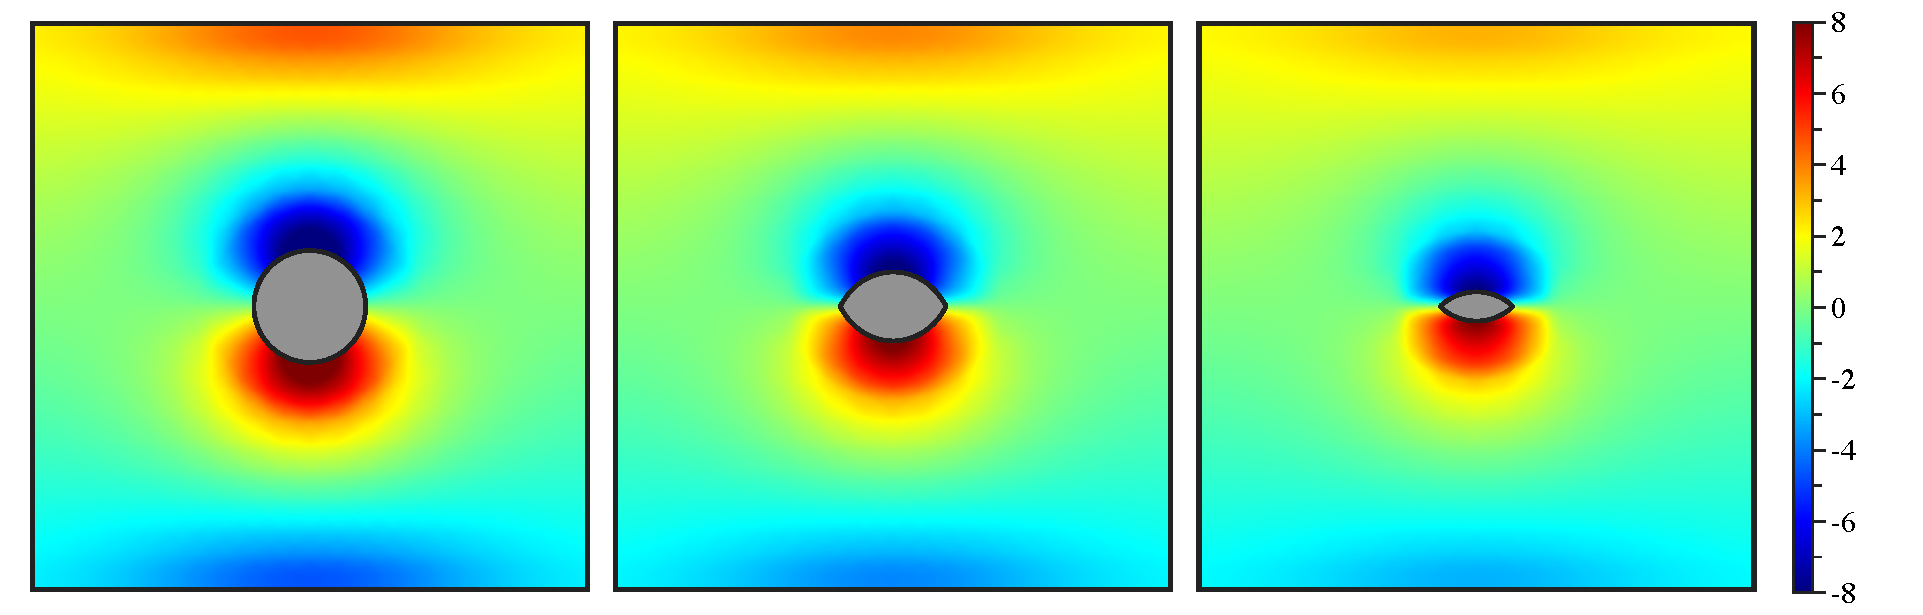
\includegraphics[width = 0.80 \textwidth]{./figs/01bodseq.pdf}
\caption{\label{01bodseq} A single body eroding in Stokes flow. As the
body erodes, it develops a corner at its front and rear stagnation
points, while remaining for-aft symmetric due to time-reversibility.
Color indicates the vorticity of the surrounding flow, which, when
evaluated on the boundary, gives the local shear stress. In this
simulation, we use $N_\iin = 1024$ discretization points on the body,
$N_\out = 1024$ points on the outer boundary, a time-step of $\Dt =
1E-6$, and smoothing parameters of $\eps = 10/1024$ and $\sigma =
10/1024$.}
\end{center}
\end{figure}
 %^^^^^^^^^^^^^^^^^^^^^^^^^^^^^^%
% Figure from datafile 01circ1024aa;
% Uses 01circ1024.in with epsfac = 10, sigfac = 10, dt = 1e-6, fixarea = 0, fixpdrop = 0

Fig.~\ref{01bodseq} shows the erosion of a single body, numerically
simulated with $N_\iin = 1024$ discretization points and shown at three
evenly spaced times. Here, color represents the vorticity of the
surrounding flow, which, when evaluated on the boundary, indicates the
shear stress and thus the local erosion rate. As seen in the left-most
snapshot, the body is initially circular and has the strongest vorticity
above and below it. The flow is for-aft symmetric as a result of the
time-reversibility of the Stokes equations, with vorticity vanishing at
the body's front and rear stagnation points. At the next instance, the
body has lost material due to erosion, but remains for-aft symmetric due
to the flow symmetry. The greatest material loss has occurred at the
body's top and bottom, where shear is strongest. Interestingly, the body
has developed well-defined corners at its front and rear stagnation
points. This geometric feature is a consequence of the erosion law,
which depends on the {\em absolute} shear stress: wherever the stress
vanishes, $\atau$ exhibits a corner, which manifests as a corner in the
geometry. As shown in the third snapshot, this corner persists as the
bodies becomes even more slender while wasting away. In this simulation,
the body completely vanishes at a final time of $t_f = 1.79E-2$.

To better understand the shape evolution, Fig.~\ref{shrink_intface}(a)
shows several superimposed interfaces at evenly spaced times. The
interfaces are color-coded by normalized time $t/t_f$. The body seems to
converge to a shape that resembles an American football---a fairly
slender, for-aft symmetric shape with corners at the front and back.
Fig.~\ref{shrink_intface}(b) shows how the absolute shear stress,
$\atau$, is distributed along each of these interfaces. The normalized
arc length $s/L$ runs counterclockwise around the body, with $s/L = 0$
corresponding to the rear stagnation point and $s/L = 0.5$ the front
stagnation point. At early times (yellow to orange), the stress is
distributed non-uniformly, with highest values at the top and bottom of
the body. As time proceeds, though, the stress becomes more evenly
distributed along the body's surface (red). As the body nears the final
stages of erosion (dark red), the stress actually becomes slightly
higher near the stagnation points. A close look reveals that {\em at}
the stagnation points, the stress always vanishes, though in a region
that becomes increasingly narrow.

%^^^^^^^^^^^^^^^^^^^^^^^^^^^^^^%
\begin{figure}%[htbp]
\begin{center}
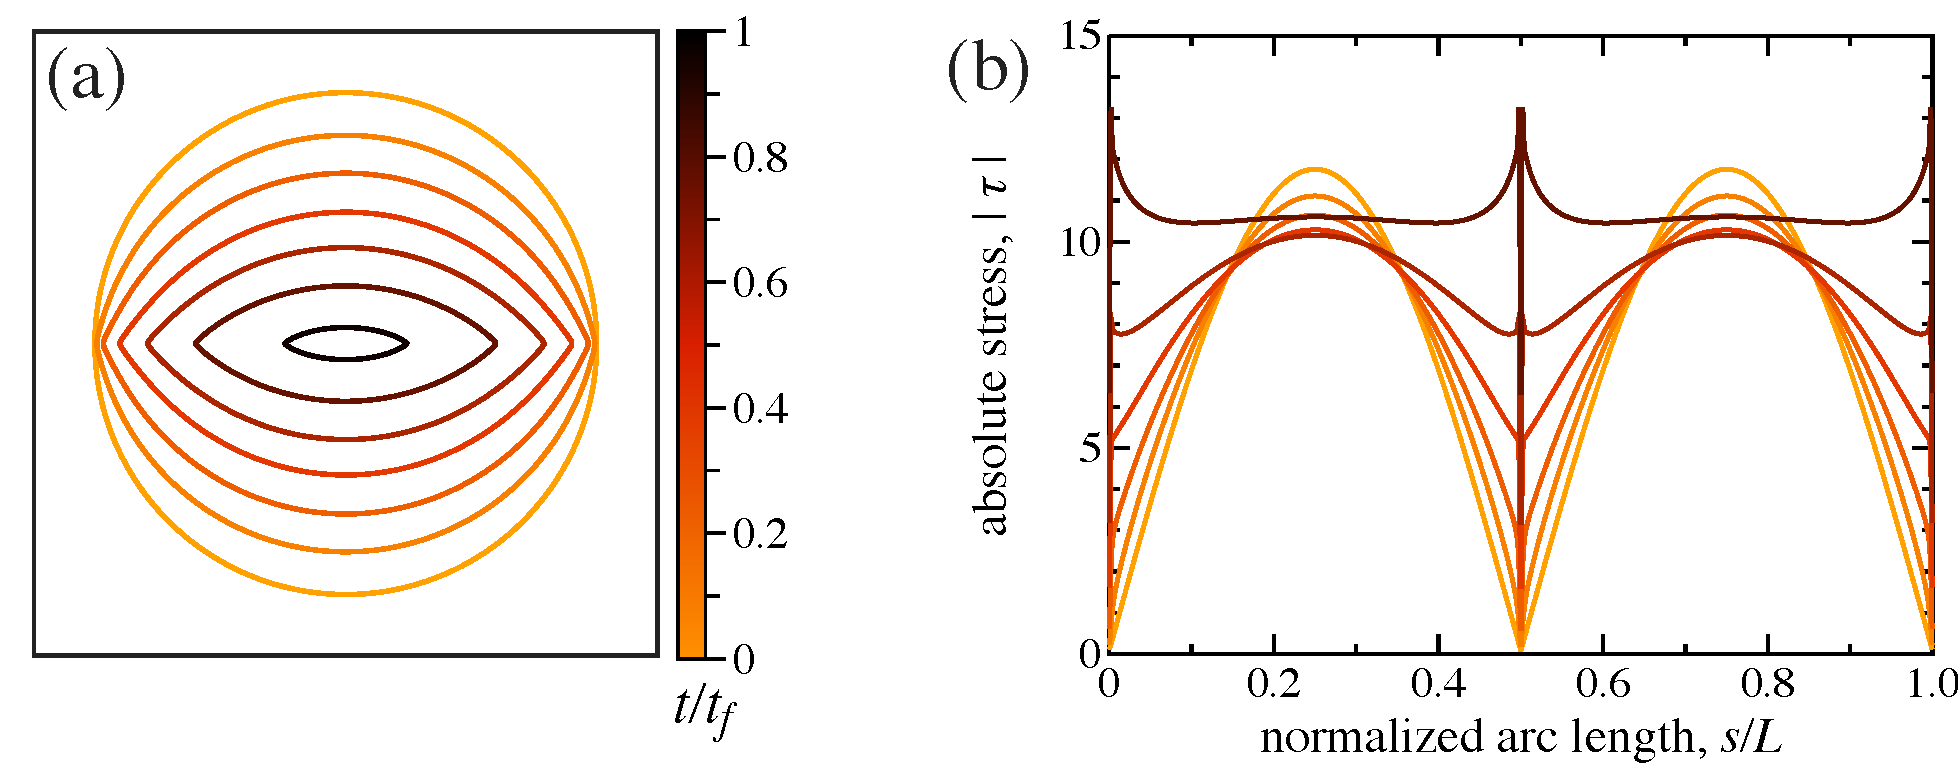
\includegraphics[width = 0.75 \textwidth]{./figs/shrink_intface.pdf}
\caption{\label{shrink_intface} Shape and stress evolution. (a)
Interfaces of the eroding body from Fig.~\ref{01bodseq} at evenly-spaced
time intervals. Color indicates normalized time, $t/t_f$, where $t_f =
1.79E-2$ is the time at which the body completely vanishes. (b) The
distribution of absolute shear stress, $\atau$, along each of these
interfaces. Normalized arc length, $s/L$, runs counterclockwise from the
rear stagnation point. The stress initially varies over the body's
surface, but becomes more uniform over time.}
\end{center}
\end{figure}
 %^^^^^^^^^^^^^^^^^^^^^^^^^^^^^^%
% Figure from datafile 01circ1024aa;
% Uses 01circ1024.in with epsfac = 10, sigfac = 10, dt = 1e-6, fixarea = 0, fixpdrop = 0

\subsection{Scaling law for the vanishing rate}

Interestingly, a brief look at Fig.~\ref{shrink_intface}(a) reveals that
the spacing between successive interfaces becomes larger as the body
shrinks, suggesting that the overall shear stress is growing. Of course,
such a relationship is consistent with the well-known 3D Stokes drag
law, $\tau \sim \mu \umax / L$, since stress is inversely proportional
to body scale $L$. This law must be modified in two dimensions, though.
The modification (made non-trivial by subtleties of the Stokes paradox)
can be correctly deduced by noting that, as the body vanishes, its drag
must be consistent with slender-body theory. For a slender body in flow
perpendicular to its long-axis $W \gg L$, the drag is proportional to
$\mu \umax W/ \log(W/L)$. This relationship implies that, for a 2D
cross-section perpendicular to the long axis, the stress (per unit $W$)
can be estimated by
\begin{align}
  \label{eqn:stresslaw}
  \tau \sim \frac{\mu \umax}{L \log(W/L)}.
\end{align}
In interpreting our 2D simulations, we will treat $W$ as fixed with the
requirement $W \gg L$.

Now, the body's rate of area reduction is given by integrating the
absolute shear stress around the boundary
\begin{align*}
  \dot{A} = \int_{\gamma} \atau \, ds \, ,
\end{align*}
giving the exact relationship
\begin{align*}
  \dot{A} = \mean{\atau} L \, .
\end{align*}
Thus, the area-loss rate is given by the product of the mean shear
$\mean{\atau}$ and the total perimeter $L$. Inserting the scaling
law~\eqref{eqn:stresslaw} gives
\begin{align*}
  \dot{A} \sim \frac{\mu \umax}{\log(W/L)} \, .
\end{align*}
Noting that $A \sim L^2$ allows one to solve the ODE to determine how the body area changes with time
\begin{align*}
  A (1 - \log A) = \areaconst (t_f - t)
\end{align*}
where $c_A$ is a constant.
This is an {\em implicit} relationship for how the area scales down in time during erosion.
In Fig.~6a, we show the body area as a function of time measured in the simulation
against the above scaling law with $\areaconst = 0.42$.

\todo[inline]{Explain the drag here too}

%^^^^^^^^^^^^^^^^^^^^^^^^^^^^^^%
\begin{figure}%[htbp]
\begin{center}
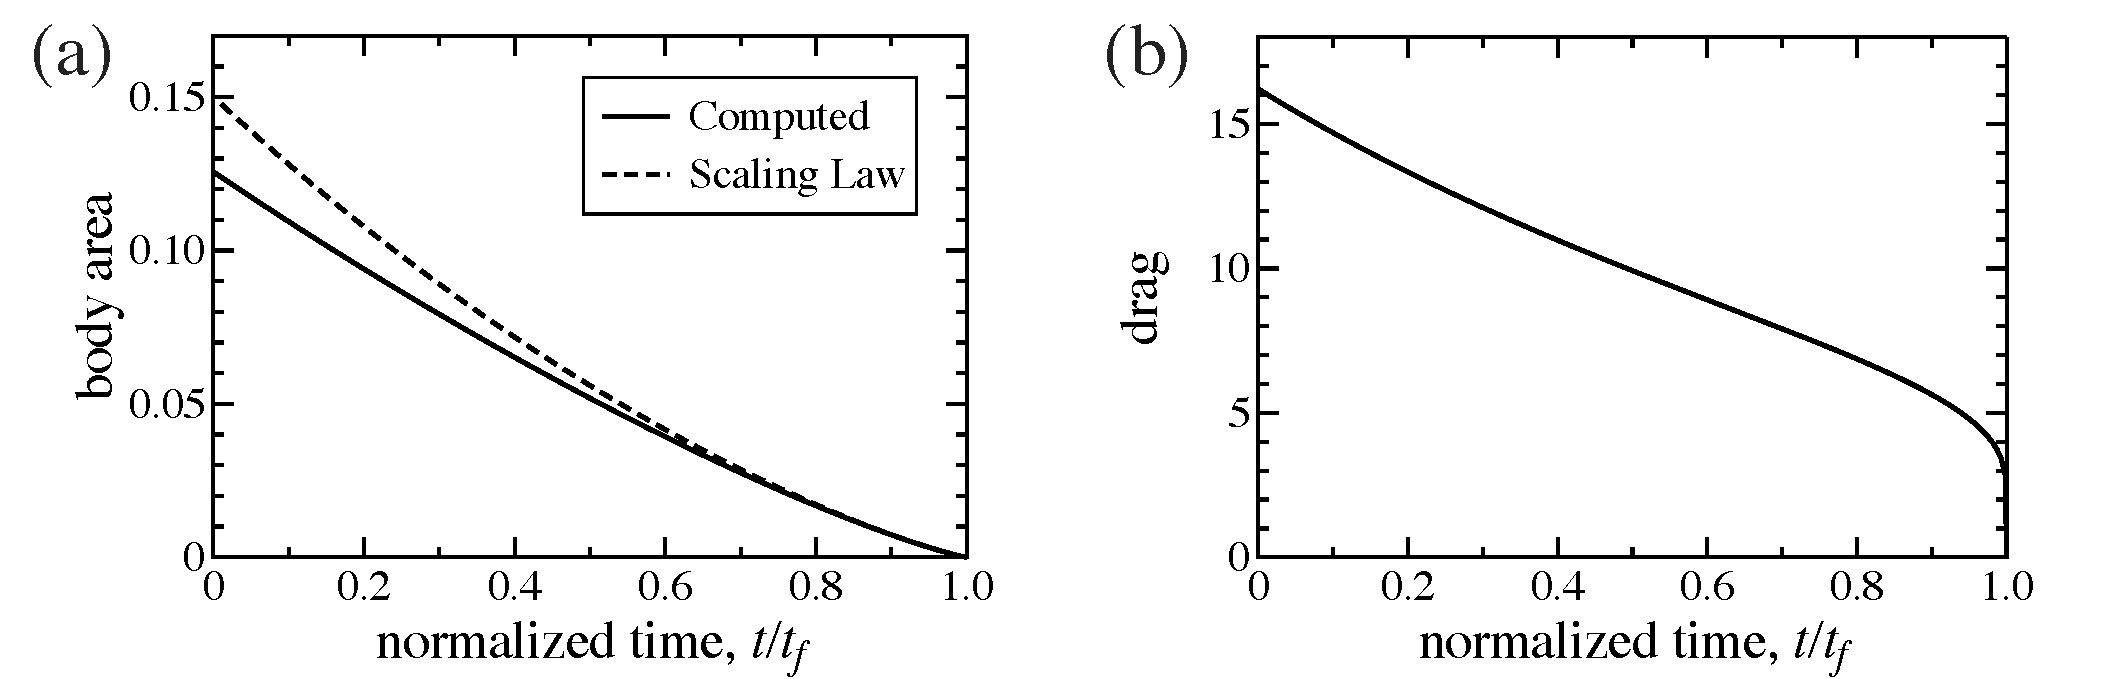
\includegraphics[width = 0.8 \textwidth]{./figs/area_drag.pdf}
\caption{One body}
\label{}
\end{center}
\end{figure}
 %^^^^^^^^^^^^^^^^^^^^^^^^^^^^^^%
% Figure from datafile 01circ1024aa;
% Uses 01circ1024.in with epsfac = 10, sigfac = 10, dt = 1e-6, fixarea = 0, fixpdrop = 0

\subsection{The limiting shape}

With the vanishing rate understood, we now seek to quantify the limiting
shape observed in Fig.~\ref{shrink_intface}a.

% Pozrikidis page 239: symmetric flow.
Certain features of this shape can be predicted analytically by
appealing to the principal of uniform stress distribution. In
particular, consider the angle formed at the front and rear stagnation
points. In long time, the stress becomes uniform, in particular in a
small vicinity of this front angle in which body curvature can be
ignored. Zooming in on the front angle, we can consider the problem of
Stokes flow around an infinite wedge of opening angle $\oangle$. Exact
solutions can be obtained to this problem via separation of variables in
polar coordinates $(r, \theta)$~\cite{poz1997}. In this section alone,
$\theta$ denotes the polar angle and not the tangent angle of the body.
The corresponding stream function is assumed to take the form $\psi =
r^{\lambda}f(\theta)$, with $\Delta^2 \psi = 0$, which gives the 4th
order ODE~\cite{poz1997}
\begin{align*}
  f'''' + 2(\lambda^2 - 2 \lambda + 2)f'' + \lambda^2(\lambda-2)^2 f = 0
\end{align*}
This ODE is subject to no-slip boundary conditions along the wedge
$f(\thb) = f'(\thb) = 0$, where $\thb = \pi - \oangle/2$, along with the
condition of odd-symmetry $f(0) = f''(0) = 0$ (corresponding to up-down
symmetry of the flow).  The corresponding shear stress evaluated on the
surface of the wedge is $\tau = \mu r^{\lambda-2} f''(\thb)$. Thus, the
wedge of uniform stress corresponds to $\lambda = 2$. For this value,
the solution for $f$ satisfying odd symmetry is
\begin{align*}
  f(\theta) = B \sin (2 \theta) + C \theta
\end{align*}
Imposing the no-slip boundary conditions gives the condition
\begin{align*}
  \sin(2 \thb) - 2 \thb \cos(2 \thb) = 0
\end{align*}
which has a solution $\thb \approx 129$ degrees. This gives an opening
angle of $\oangle = 2(\pi - \thb) \approx 102$ degrees.

We aim to measure the opening angle in our simulation, but, curiously,
the body vanishes before a steady-state is definitively reached. To
obtain the true terminal shape, we could restart our simulation with the
final eroded body scaled up and iterate this process until reaching
steady state. A simpler solution, though, is to remove the effect of
shrinking during the erosion process by simply modifying the normal
velocity $\Vn$ to have zero mean
\begin{align*}
  \Vn \leftarrow \Vn - \mean{\Vn}
\end{align*}
This modification allows erosion to modify the body shape as it would
normally, but artificially keeps the area of the body fixed. We show in
Fig.~\ref{fixed_intface}a several interfaces at equally spaced times.
Notice the body obtains the slender, football shape seen previously, but
here more precision is available. We also show in
Fig.~\ref{fixed_intface}b the stress, showing that the stress becomes
much more evenly distributed as time proceeds. In this figure, time is
normalized by the same vanishing time $t_f = 1.79E-2$ as the simulation
shown in Fig.~\ref{shrink_intface}. Curiously, about 3 multiples of
$t_f$ are required to reach a visually satisfying stead-state. This is
very much in contrast to previous studies of erosion in high-Reynold's
number flows, in which a reasonable steady-state was reached before the
body vanished~\cite{moo-ris-chi-zha-she2013}.

%^^^^^^^^^^^^^^^^^^^^^^^^^^^^^^%
\begin{figure}%[htbp]
\begin{center}
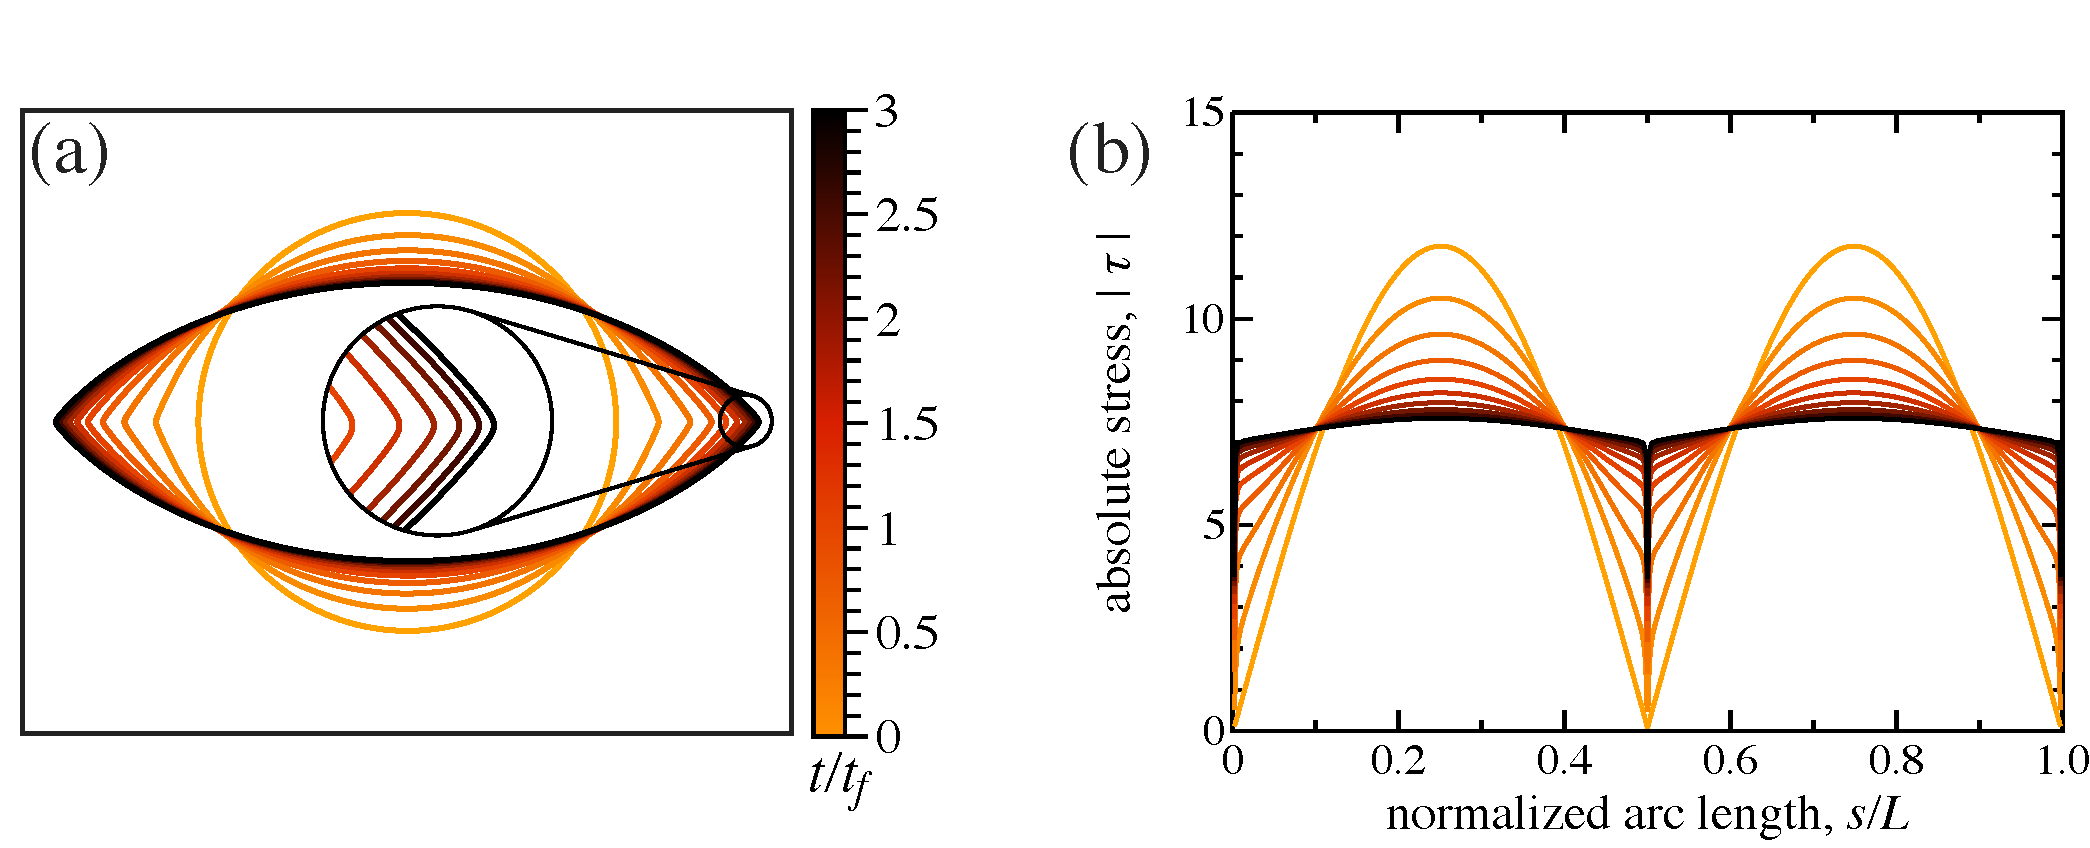
\includegraphics[width = 0.8 \textwidth]{./figs/fixed_intface.pdf}
\caption{One body fixed area}
\label{fixed_intface}
\end{center}
\end{figure}
 %^^^^^^^^^^^^^^^^^^^^^^^^^^^^^^%
% Figure from datafile 01circ1024c5
% Uses 01circ1024.in with epsfac = 5, sigfac = 5, dt = 2e-4, fixarea = 1, fixpdrop = 0

The fixed-area simulations allow us to make precise measurements of the
body's opening angle and aspect ratio as displayed in
Fig.~\ref{fig:arangle}. Fig.~\ref{fig:arangle}a shows the aspect
ratio, defined as the body's horizontal compared to its vertical width.
The initial circular geometry has an aspect ratio of unity. As erosion
causes the body to become more slender, the aspect ratio increases and
tends to a value of $2.7$ in long time. Fig.~\ref{fig:arangle}b shows
the body's opening angle, which we measure by fitting the tangent angle
$\theta(\alpha)$ with a 7th degree polynomial over a region excluding
the front/rear stagnation point (where there is high curvature that
approximates an angle). The polynomial fit is then extrapolated to the
stagnation point to get an angle estimate (subject to some uncertainty,
which we estimate below). As seen in Fig.~\ref{fig:arangle}a, the
opening angle is initially $180^\circ$, corresponding to the initially
circular geometry. Erosion causes the angle to form after a short time,
and the angle becomes increasingly sharp as it converges to the value
$102^\circ$ in long time. This coincides exactly with the valued
predicted by our local solutions.

\todo[inline]{Also point to figure 7a, with the smoothed out corner}

%^^^^^^^^^^^^^^^^^^^^^^^^^^^^^^%
\begin{figure}%[htbp]
\begin{center}
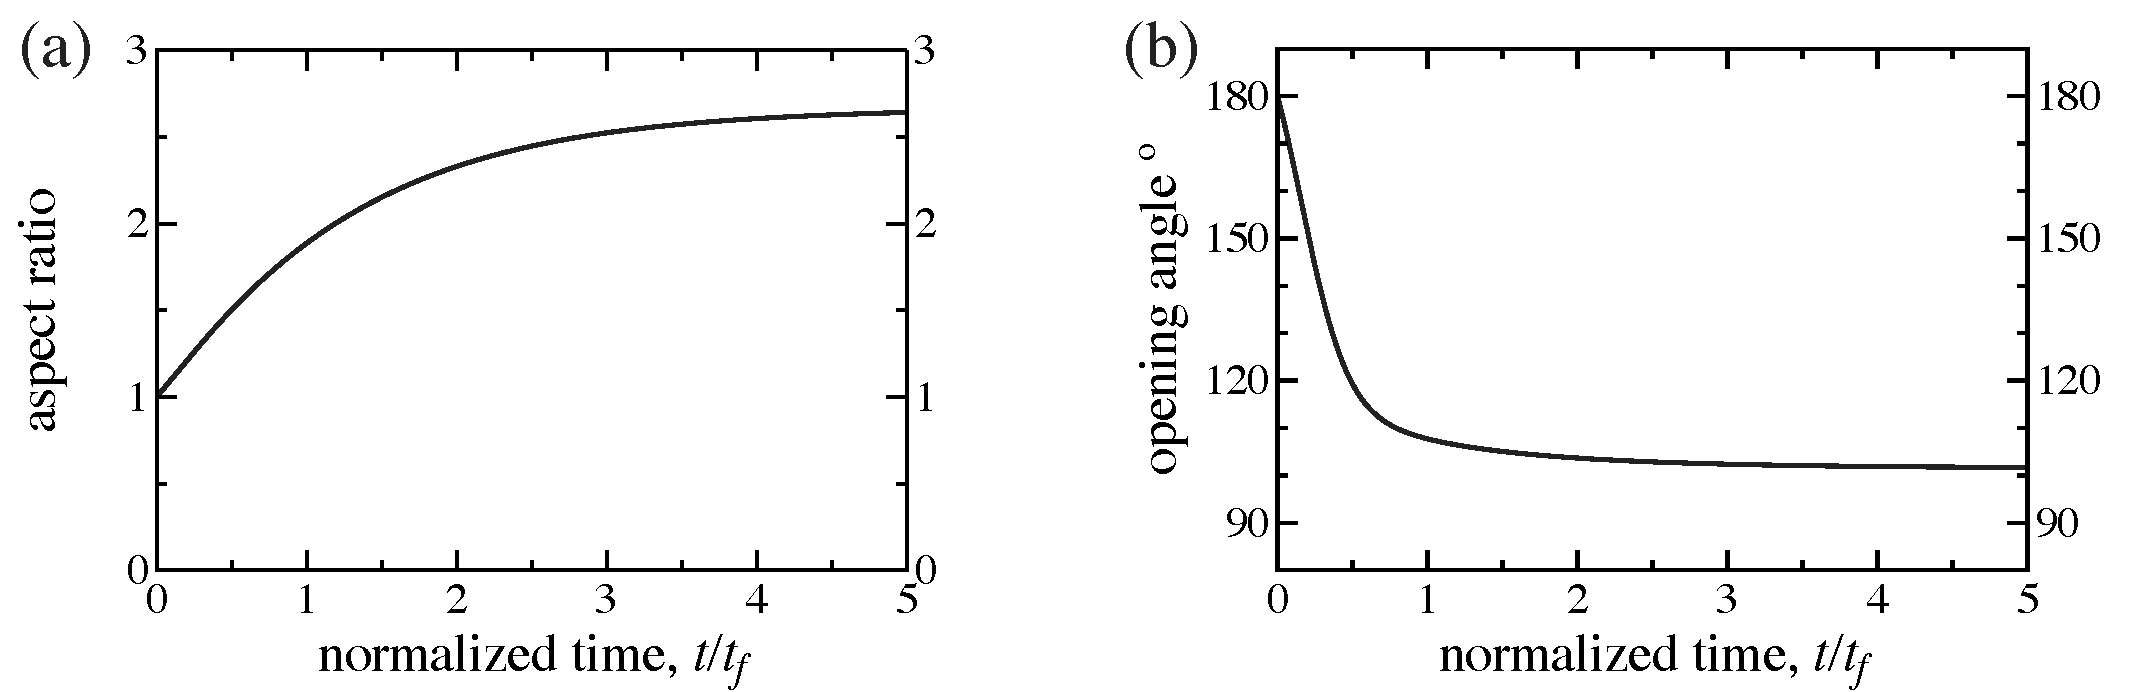
\includegraphics[width = 0.8 \textwidth]{./figs/arangle.pdf}
\caption{Aspect ratio and opening angle}
\label{fig:arangle}
\end{center}
\end{figure}
 %^^^^^^^^^^^^^^^^^^^^^^^^^^^^^^%
% Figure from datafile 01circ1024c5
% Uses 01circ1024.in with epsfac = 5, sigfac = 5, dt = 2e-4, fixarea = 1, fixpdrop = 0

To examine the influence of the smoothing parameters, $\eps$ and
$\sigma$, we show in Table~\ref{table:arangle} the measurements of
aspect ratio and opening angle for different simulations. We fix the
total number of discretization points at $N_\iin = 1024$ and
sequentially reduce the smoothing with $\eps$ and $\sigma$ always equal.
We choose the values $20/1024$, $10/1024$, and $5/1024$. Roughly, this
corresponds to smoothing over the nearest 20, 10, and 5 grid points
respectively. As seen in the table, the aspect ratio converges to a
values of $2.65$ and the opening angle converges to $102^{\circ}$. We
also estimate the uncertainty in the angle measurements by varying the
region of the polynomial fit and the degree of the fit. As shown in the
table, as the smoothing parameters are reduced, the angle measurements
become more
precise.

% Table
%^^^^^^^^^^^^^^^^^^^^^^^^^^^^^^%
\begin{table}%[htbp]
\begin{center}
\caption{Final aspect ratio and opening angle
} 
\vspace{0.3 pc}
\label{table:arangle}
\begin{tabular}{c c c}
\hline
\hspace{0.5pc} smoothing parameters: $\eps$ and $\sigma$
\hspace{0.5pc} & final aspect ratio 
\hspace{0.5pc} & final opening angle \\
\hline
20/1024		& 2.55	& $110^\circ \pm 6^\circ$	\\
10/1024		& 2.62	& $104^\circ \pm 4^\circ$	\\
5/1024		& 2.65	& $102^\circ \pm 2^\circ$	\\
\hline
\end{tabular}
\end{center}
\end{table}
 %^^^^^^^^^^^^^^^^^^^^^^^^^^^^^^%
% npts = 1024




\vsp{30}








% Table
%^^^^^^^^^^^^^^^^^^^^^^^^^^^^^^%
\begin{table}%[htbp]
\begin{center}
\caption{Convergence test: the stopping time is $t_s =$ 1E-2, which is
56\% of the vanishing time.  GOOD TERM: Cauchy-convergence.} 
\caption{Convergence test: the stopping time is $t_s =$ 1E-2, which is
56\% of the vanishing time.
} 
\vspace{0.3 pc}
\label{convtab}
\begin{tabular}{c l l}
\hline
\hspace{0.5pc} $\Delta t/t_s$
\hspace{0.5pc} & error 
\hspace{0.5pc} & order \\
\hline
1/100	& 4.69E-6		& --		\\
1/200	& 1.26E-6		& 1.90	\\
1/400	& 3.26E-7		& 1.95	\\
1/800	& 8.28E-8		& 1.98	\\
1/1600	& 2.09E-8		& 1.99	\\
1/3200	& 5.26E-9		& 1.99	\\
1/6400	& --			& --		\\
\hline
\end{tabular}
\end{center}
\end{table}
 %^^^^^^^^^^^^^^^^^^^^^^^^^^^^^^%
% Parameters in this test are: 01circ256, nits = 7, dt0 = 1e-4, tfin = 1e-2
% epsfac = 10, sigfac = 10, fixarea = 0, fixprdop = 0

In the table, we measure the error in the shape by computing the L2-difference of the interfaces.



% NEWPAGE
\newpage


Runs to do
\begin{itemize}
  \item Single body
  \begin{itemize}
    \item Aspect ratio and opening angle
    \item Drag and resistivity
    \item Anisotropy
    \item Vorticity
  \end{itemize}
  \item $\bigO(5)$ bodies
  \begin{itemize}
    \item Drag and resistivity
    \item Anisotropy
    \item Long channels between flat faces
    \item Vorticity
  \end{itemize}
  \item $\bigO(50)$ bodies
  \begin{itemize}
    \item Drag and resistivity
    \item Anisotropy
    \item Vorticity
  \end{itemize}
\end{itemize}


%%%%%%%%%%%%%%%%%%%%%%%%%%%%%%%%%%%%%%%%%%%%%%%%%%%%%%%%%%%%%%%%%%%%%%%
\section{Conclusions\label{s:conclusions}}


%%%%%%%%%%%%%%%%%%%%%%%%%%%%%%%%%%%%%%%%%%%%%%%%%%%%%%%%%%%%%%%%%%%%%%%
\paragraph{\bf Acknowledgments} The authors would like to thank Manas
Rachh for supplying the FMM for the Stokes double-layer potential.


%%%%%%%%%%%%%%%%%%%%%%%%%%%%%%%%%%%%%%%%%%%%%%%%%%%%%%%%%%%%%%%%%%%%%%%
\begin{appendices}
\section{Error estimates for near-singular integration \label{A:AppendixA}} 
\end{appendices}


\bibliographystyle{plainnat} 
\bibliography{refs}
\biboptions{sort&compress}
\end{document}


